\documentclass[12pt]{article}
\usepackage{MicSheets}


\begin{document}
\title{AQP Example Sheets}
\author{Feiyang Chen}
\date{Michaelmas 2020}
\maketitle
\thispagestyle{empty}
\tableofcontents
\newpage
\section{}
\subsection{} \( \hat{H}\) is Hermitian
\subsubsection{} \begin{align*}
    \hat{H} \ket{\psi_1} &=  E_1 \ket{\psi_1}\\
    \hat{H} \ket{\psi_2} &=\, E_2 \ket{\psi_2}\\
    \bra{\psi_1} \hat{H} \ket{\psi_2} - \bra{\psi_1} \hat{H}
    \ket{\psi_2} &= 0\\
    (E_1^* - E_2)\braket{\psi_1|\psi_2} &=  0\\
    E_1\neq E_2 \implies\; \braket{\psi_1|\psi_2} &=  0    \implies\, \text{orthogonal eigenstates}  
\end{align*}
\subsubsection{} \begin{gather*}
    \hat{A} \ket{\psi_1} =\ket{\psi_2};\;  \hat{A}
    \ket{\psi_2} =\ket{\psi_1}\\
    \hat{A}\left(\frac{1}{\sqrt{2}}(\ket{\psi_1} + \ket{\psi_2})\right) = \frac{1}{\sqrt{2}} (\ket{\psi_2} + \ket{\psi_1}) = \ket{a_1}\\
    \hat{A}\left(\frac{1}{\sqrt{2}}(\ket{\psi_1} - \ket{\psi_2})\right) = \frac{1}{\sqrt{2}} (\ket{\psi_2} - \ket{\psi_1}) = \ket{a_2} 
\end{gather*}
\begin{center} \begin{tabular}{cc} 
    eigenstates & eigenvalues  \\ 
    \( \ket{a_1} \) &  1\\ 
    \( \ket{a_2} \) & -1\\
\end{tabular} \end{center}
\subsubsection{} At $t=0$ after measuring $A$, \[
    \ket{\psi(0)} = \ket{a_2} = \frac{1}{\sqrt{2}}( \ket{\psi_1} - \ket{\psi_2} )  \]
    \begin{align*}
        \ket{\psi(t)} &=  \frac{1}{\sqrt{2}}( e^{ -\frac{i\,t}{\hbar}E_1}\ket{\psi_1}
        - e^{ -\frac{i\,t}{\hbar}E_2}\ket{\psi_2}) \\
        P(t) &= \abs{\braket{a_2|\psi(t)}^2 }\\
        &= \frac{1}{4} \abs{ e^{ -\frac{i\,t}{\hbar}E_2} + e^{\frac{i\,t}{\hbar}E_1}}^2\\
        &= \frac{1}{4} \left((\cos \frac{E_2t}{ \hbar} + \cos \frac{E_1 t}{ \hbar})^2 +
        (\sin \frac{E_2t}{ \hbar} + \sin \frac{E_1 t}{ \hbar})^2\right)\\
        &=\, \frac{1}{2} + \frac{1}{2}\left(\cos \frac{E_2t}{ \hbar}\cos \frac{E_1t}{ \hbar} +
        \sin \frac{E_2t}{ \hbar}\sin \frac{E_1t}{ \hbar}\right)\\
        &= \frac{1}{2} + \frac{1}{2}\cos \frac{(E_1 - E_2)t}{ \hbar}\\
        &= \cos^2\frac{(E_1 - E_2)t}{2 \hbar}\, 
    \end{align*}
\subsection{} \begin{align*}
j=&\frac{\hbar}{2mi} \pqty{\psi^* \pdv{\psi }{x} - \psi \pdv{\psi^*}{t}}\\
=&\frac{\hbar}{2mi} \left[\pqty{A^*e^{ - ikx} + B^*e^{ikx}}\pqty{ikAe^{ikx} - ik Be^{ -ikx}} \right.\\
&\qquad\left.+\pqty{Ae^{ikx} + Be^{ -ikx}}\pqty{ -ikA^*e^{ -ikx} + ik B^*e^{ikx}}\right]\\
=& \frac{\hbar}{2mi} \bqty{2\pqty{ik A^*A - ikB^*B} + 0}\\
=& \frac{\hbar k}{m} \pqty{\abs{A}^2 - \abs{B}^2}
\end{align*}
\subsection{}
\subsubsection{} \begin{align*}
    a^\dagger \ket{\psi_n} &= \sqrt{n + 1}\ket{\psi_{n + 1}}\\
    a \ket{\psi_n} &=  \sqrt{n}\ket{\psi_{n - 1}}\\
    \braket{x}_{\psi_n} &= \bra{\psi_n} x \ket{\psi_n}\\
    &= \frac{\sqrt{2m \hbar\omega }}{2m\omega }  \bra{\psi_n} (a^\dagger + a) \ket{\psi_n}\\
    &= \frac{\sqrt{2m \hbar\omega }}{2m\omega }  \bra{\psi_n} (\sqrt{n + 1}
    \ket{\psi_{n + 1}} +\sqrt{n} \ket{\psi_{n -
    1}})\\
    &= 0\;  \text{by orthogonality of eigenstates}\\
    \braket{p}_{\psi_n} &= \bra{\psi_n} p
    \ket{\psi_n}\\ 
    &= \frac{i\sqrt{2m \hbar\omega }}{2}
    \bra{\psi_n} (a^\dagger - a) \ket{\psi_n}\\ 
    &= \frac{i\sqrt{2m
    \hbar\omega }}{2} \bra{\psi_n} (\sqrt{n + 1}
    \ket{\psi_{n + 1}} -\sqrt{n} \ket{\psi_{n - 1}})\\ 
    &= 0\;\text{by orthogonality of eigenstates}
\end{align*}
\subsubsection{}  \begin{align*}
    \hat{H} &=  \frac{1}{2} m\omega^2 \hat{x}^2 + \frac{\hat{p}^2}{2m}\\
    &= (a^\dagger a + \frac{1}{2}) \hbar\omega\\
    \hat{H} \ket{\psi_n} &= \hbar\omega (\sqrt{n\, n} + \frac{1}{2})
    \ket{\psi_n}\\
    &= (n + \frac{1}{2}) \hbar\omega \\
    \bra{\psi_n} V \ket{\psi_n} &= (\frac{\sqrt{2m \hbar\omega} }{2m\omega } )^2\:  \frac{m\omega^2}{2}\bra{\psi_n} (a^\dagger + a)^2                \ket{\psi_n} \\
    &= \frac{1}{4} \hbar\omega\bra{\psi_n} (a^\dagger a + a a^\dagger ) \ket{\psi_n} \\
    &= \frac{1}{4} \hbar\omega\bra{\psi_n} (n + n + 1) \ket{\psi_n} \\
    &= \frac{1}{2} (n + \frac{1}{2}) \hbar\omega \\
    \bra{\psi_n} \frac{\hat{p}^2}{2m} \ket{\psi_n} &= - \frac{1}{4} \hbar\omega \bra{\psi_n}
    (a^\dagger - a)^2 \ket{\psi_n} \\ &= \frac{1}{4} \hbar\omega \bra{\psi_n} (a^\dagger a + a a^\dagger )
    \ket{\psi_n} \\ &= \frac{1}{4} \hbar\omega
    \bra{\psi_n} (n + n + 1) \ket{\psi_n} \\ &=
    \frac{1}{2} (n + \frac{1}{2}) \hbar\omega
\end{align*}
\subsubsection{} \begin{align*}
    (\Delta x)^2 &=\, \braket{x^2} - \braket{x}^2\\
    &= \frac{1}{2}(n + \frac{1}{2}) \hbar\omega\, \frac{2}{m\omega^2} \\&=  (n + \frac{1}{2}) \frac{\hbar}{m\omega }\\
    (\Delta p)^2 &=\,
    \braket{p^2} - \braket{p}^2\\ &= \frac{1}{2}(n + \frac{1}{2})
    \hbar\omega\, 2m \\&=  (n + \frac{1}{2})
    \hbar m\omega \\
    \Delta x \Delta p &=(n + \frac{1}{2}) \hbar
\end{align*}
\subsection{} It is easy to compute \begin{align*}
\comm{L_x}{L_y} = i\frac{\hbar^2}{2} \begin{pmatrix} 1&0&-1\\
0&0&0\\
1&0&-1\end{pmatrix} - i\frac{\hbar^2}{2}\begin{pmatrix} -1&0&-1\\
0&0&0\\
1&0&1 \end{pmatrix} = i\hbar L_z
\end{align*}
Similarly, 
\begin{align*}
\comm{L_y}{L_z} &= i\frac{\hbar^2}{\sqrt{2}} \begin{pmatrix} 0&0&0\\
1&0&1\\
0&0&0\end{pmatrix} - i\frac{\hbar^2}{\sqrt{2}}\begin{pmatrix} 0&-1&0\\
0&0&0\\
0&- 1&0 \end{pmatrix} = i\hbar L_x &\comm{L_z}{L_x}&= i\hbar L_y
\end{align*}
These operators:\begin{itemize}
\item are Hermitian;
\item act on vectors in \(\mathbb{R}^3 \implies \) have 3 degrees of freedom for \(m_l =- 1,0,1\) respectively;
\item satisfy commutation relations;
\end{itemize}
Therefore they are suitable as angular momentum operators.
\begin{align*}
\hat{H} &=  \frac{\hbar^2}{2I_x}\begin{pmatrix} 1&0&1\\0&2&0\\subsection{}&0&1 \end{pmatrix} - \frac{\hbar^2}{2I_y} \begin{pmatrix} - 1&0&1\\0&- 2&0\\subsection{}&0&- 1 \end{pmatrix} + \frac{\hbar^2}{I_z}\begin{pmatrix}1&0&0\\0&0&0\\0&0&1  \end{pmatrix}\\
\hat{H} &=  \frac{\hbar^2}{2}
\begin{pmatrix} 
    \frac{1}{I_x} + \frac{1}{I_y} + \frac{2}{I_z}&0&\frac{1}{I_x} - \frac{1}{I_y}\\
    0&\frac{2}{I_x} + \frac{2}{I_y}&0\\
    \frac{1}{I_x} - \frac{1}{I_y}&0&\frac{1}{I_x} + \frac{1}{I_y} + \frac{2}{I_z}
\end{pmatrix} 
\end{align*}
The energy eigenstates and eigenvalues are 
\begin{align*}
\frac{1}{\sqrt{2}}&\bqty{\ket{Y_{11}} + \ket{Y_{1 -1}} } &\frac{1}{\sqrt{2}}&\bqty{\ket{Y_{11}} - \ket{Y_{1 -1}} }&&\ket{Y_{10}}\\ 
\hbar^2&\bqty{\frac{1}{I_x} + \frac{1}{I_z}} &\hbar^2&\bqty{\frac{1}{I_y} + \frac{1}{I_z}} & \hbar^2&\bqty{\frac{1}{I_x} + \frac{1}{I_y}}
\end{align*}
\subsection{} Define 
\begin{align*}
S_{\theta,\phi }&\equiv \frac{\hbar}{2}\pqty{\sin \theta \cos \phi \begin{pmatrix} 0&1\\subsection{}&0 \end{pmatrix}  + \sin \theta \sin \phi  \begin{pmatrix} 0&-i\\i&0 \end{pmatrix} + \cos \theta \begin{pmatrix} 1&0\\0&- 1 \end{pmatrix}}\\
&= \frac{\hbar}{2} \begin{pmatrix} \cos \theta &\sin \theta (\cos \phi - i \sin \phi )\\ \sin \theta \pqty{\cos \phi + i\sin \phi }&- \cos \theta  \end{pmatrix}
\end{align*}
Its eigenvalues are solutions to the equation \begin{gather*}
\pqty{\cos \theta - \frac{2s}{\hbar}}\pqty{\cos \theta + \frac{2s}{\hbar}} + \sin^2 \theta \pqty{\cos^2 \phi+ \sin^2 \phi } = 0\\
1 - \pqty{\frac{2s}{\hbar}}^2 = 0\\
s = \pm \frac{\hbar}{2}
\end{gather*}
and eigenstates can be worked out by \begin{gather*}
\begin{pmatrix} \cos \theta &e^{ - i\phi }\sin \theta \\ e^{i\phi }\sin \theta &- \cos \theta  \end{pmatrix} \begin{pmatrix} \psi_1\\ \psi_2 \end{pmatrix} = \pm 1 \begin{pmatrix} \psi_1\\ \psi_2 \end{pmatrix} \\
\begin{pmatrix} \psi_1\\ \psi_2  \end{pmatrix} = \begin{pmatrix} e^{ - \frac{i\phi}{2}} \cos \frac{\theta}{2}\\e^{  \frac{i\phi}{2}} \sin \frac{\theta}{2} \end{pmatrix} \text{ or } \begin{pmatrix} e^{ - \frac{i\phi}{2}} \sin \frac{\theta}{2}\\e^{  \frac{i\phi}{2}} \cos \frac{\theta}{2} \end{pmatrix}
\end{gather*}
The spin eigenstates for \( + x, - x, + y, - y\) are therefore \begin{align*}
\frac{1}{\sqrt{2}}\begin{pmatrix} 1\\subsection{} \end{pmatrix}&& \frac{1}{\sqrt{2}}\begin{pmatrix} - i\\i \end{pmatrix} &&\frac{1}{2}\begin{pmatrix} 1 - i\\subsection{} + i \end{pmatrix}&&\frac{1}{2}\begin{pmatrix} 1 + i\\subsection{} - i \end{pmatrix}
\end{align*}
respectively.
\subsection{} The energy eigenvalue equaion for any one particle gives\begin{gather*}
- \frac{\hbar^2}{2m} \pdv[2]{x} \psi + V(x)\psi = E \psi\\
\psi_n(x) = \sqrt{\frac{2}{L}}\sin \pqty{\frac{n\pi x}{L}} \quad\text{ for }x\in[0,L] \qquad 0 \text{ otherwise}
\end{gather*}
We want a wavefunction for two indistinguishable particles. Two particles in the same state $n_1=n_2$ are already exchange symmetric. For two particles in two states \(n_1 \neq n_2\),symmetrising over the spatial part gives\begin{gather*}
\Psi^{s/a}_{n_1,n_2}(x_1,x_2) = \frac{1}{\sqrt{2}}\pqty{\psi_{n_1}(x_1)\psi_{n_2}(x_2) \pm \psi_{n_2}(x_1)\psi_{n_1}(x_2)}\\
\hat{H}(x_1,x_2) \Psi^{s/a} = \frac{\hbar^2}{2m} \bqty{\pqty{\frac{n_1\pi}{L}}^2 +\pqty{\frac{n_2\pi}{L}}^2}\Psi^{s /a}
\end{gather*}
The total energy eigenvalue is \[
E =\frac{\hbar^2\pi^2}{2mL^2}\pqty{n_1^2 + n_2^2} = \pqty{n_1^2 + n_2^2} \varepsilon
\]
With \(E = 5 \varepsilon = \pqty{1^2 + 2^2}\varepsilon\)
\subsubsection{} Spin zero particles are symmetric under exchange. 
\[
\ket{\Psi(x_1,x_2)} = \frac{1}{\sqrt{2}}\bqty{\psi_{1}(x_1)\psi_{2}(x_2) + \psi_{2}(1)\psi_{1}(x_2)} = \Psi^s_{1,2}
\]
(no spin parts attached.)
\subsubsection{} Spin-\(\frac{1}{2}\) particles have overall exchange-antisymmetric wavefunctions. Spin singlets have antisymmetric spin parts so wavefunctions have to be symmetric
\[
\ket{\Psi(x_1,x_2), S_{0,0}} = \Psi^s_{1,2} \frac{1}{\sqrt{2}} \bqty{\ket{\uparrow\downarrow} - \ket{\downarrow\uparrow} }
\]
\begin{figure}[H]
\centering
\def\svgwidth{200pt}
\incfig{AQP_7s}
\caption{Approximate plot of  \(\pqty{\Psi^s(x_1,x_2)}^2\)}
\end{figure}
\subsubsection{} 3 different spin triplet states which have symmetric spin parts can be constructed, their spatial parts are antisymmetric.
\begin{align*}
\ket{\Psi(x_1,x_2), S_{1, - 1}} &=  \Psi^a_{1,2} \frac{1}{\sqrt{2}} \ket{\downarrow\downarrow}\\
\ket{\Psi(x_1,x_2), S_{1,0}} &=  \Psi^a_{1,2} \frac{1}{\sqrt{2}} \bqty{\ket{\uparrow\downarrow} + \ket{\downarrow\uparrow} }\\
\ket{\Psi(x_1,x_2), S_{1, + 1}} &=  \Psi^a_{1,2} \frac{1}{\sqrt{2}} \ket{\uparrow\uparrow}
\end{align*}
\begin{figure}[tbp]
\centering
\def\svgwidth{200pt}
\incfig{AQP_7}
\caption{Approximate plot of \(\pqty{\Psi^a(x_1,x_2)}^2\)}
\end{figure}
If the particles interacted via a repulsive interparticular potential, the energy of exchange symmetric wavefunctions would increase whereas the energy of exchange antisymmetric wavefunctions would decrease.
\subsection{} For the Quantum Harmonic Oscillator \begin{align*}
\hat{H} &=  (a^\dagger a + \frac{1}{2})\hbar\omega \\
U^\dagger  =e^{i\hat{H}t} &= \sum_{n = 0}^{\infty}e^{\frac{it}{ \hbar}(n + \frac{1}{2})\hbar\omega }\ket{n} \bra{n}\\
a(t) &=  \sum_{m,n}e^{\frac{it}{ \hbar}(m + \frac{1}{2})\hbar\omega - \frac{it}{\hbar}(n + \frac{1}{2})\hbar\omega } \ket{m}\bra{m} a(0) \ket{n} \bra{n} \\
&= \sum_{m,n}e^{it(m - n) \omega } \ket{m} \sqrt{n} \delta_{m,n - 1} \bra{n} \\
&= e^{ -i \omega t} \sum_n \sqrt{n} \ket{n - 1} \bra{n} \\
&= e^{ -i \omega t} a(0)
\end{align*}
Similarly,
\begin{align*}
a^\dagger (t) &=  \sum_{m,n}e^{i(m - n) \omega t} \ket{m} \sqrt{n + 1} \delta_{m,n + 1} \bra{n} \\
a^\dagger (t) &= e^{i \omega t} \sum_{n} \ket{n + 1} \sqrt{n + 1} \bra{n} \\
a^\dagger (t) &= e^{i \omega t} a^\dagger (0) 
\end{align*}
\begin{align*}
\hat{x} &=  \frac{\sqrt{2m \hbar\omega} }{2m\omega }  (a^\dagger(t) + a(t))\\
\dv{\hat{x}}{t} &= \frac{\sqrt{2m \hbar\omega}}{2m\omega } (i \omega a^\dagger(t) - i \omega  a(t))\\
\dv{\hat{x}}{t} &= i \frac{\sqrt{2m \hbar\omega}}{2m }  (a^\dagger(t) -  a(t)) = \frac{\hat{p}}{m} 
\end{align*}

For a general system with potential $V(x)$
\begin{align*}
\hat{x}(t) &= e^{\frac{i\,t}{\hbar}\hat{H}}\: \hat{x}^S\:  e^{ -\frac{i\,t}{\hbar}\hat{H}}\\
\dv{\hat{x}}{t} &= \frac{i}{ \hbar}  e^{\frac{i\,t}{\hbar}\hat{H}}\: \hat{H}\hat{x}^S\: e^{ -\frac{i\,t}{\hbar}\hat{H}} - \frac{i}{ \hbar} e^{\frac{i\,t}{\hbar}\hat{H}}\:  \hat{x}^S \hat{H}\: e^{ -\frac{i\,t}{\hbar}\hat{H}}\\
&= \frac{i}{ \hbar} e^{\frac{i\,t}{\hbar}\hat{H}}\: \comm{\frac{\pqty{\hat{p}^S}^2 }{2m}}{\hat{x}^S}\: e^{ -\frac{i\,t}{\hbar}\hat{H}}\\
&= \frac{i}{2m \hbar} 2 \hat{p}( - i \hbar)\\
&= \frac{\hat{p}}{m}\qquad \blacksquare
\end{align*}
Similarly,
\begin{align*}
\hat{p}(t) &= e^{\frac{i\,t}{\hbar}\hat{H}}\: \hat{p}^S\:  e^{ -\frac{i\,t}{\hbar}\hat{H}}\\
\dv{\hat{p}}{t} &= \frac{i}{ \hbar}  e^{\frac{i\,t}{\hbar}\hat{H}}\: \hat{H}\hat{p}^S\: e^{ -\frac{i\,t}{\hbar}\hat{H}} - \frac{i}{ \hbar} e^{\frac{i\,t}{\hbar}\hat{H}}\:  \hat{p}^S \hat{H}\: e^{ -\frac{i\,t}{\hbar}\hat{H}}\\
&= \frac{i}{ \hbar} e^{\frac{i\,t}{\hbar}\hat{H}}\: \comm{V^S(x)}{\hat{p}^S}\: e^{ -\frac{i\,t}{\hbar}\hat{H}}\\
&= \frac{i}{\hbar} \dv{\hat{V}(x)}{x} \,  i \hbar\\
&= - e^{\frac{i\,t}{\hbar}\hat{H}}\dv{\hat{V}^S(x)}{x} e^{ -\frac{i\,t}{\hbar}\hat{H}}
\end{align*}
\newpage
\section{}
\subsection{} For a system in a time-independent Hamiltonian, the time shift operator is \begin{align*}
    U(t,t_0) &=  e^{ -i\pqty{t - t_0}H/\hbar}\\
    U(t,t_0) &=  \sum_n \exp{ - i(t - t_0)\frac{E_n}{\hbar}} \ket{\psi_n} \bra{\psi_n} 
\end{align*}
where \(\ket{\psi_n} \) are the energy eigenstates.
\subsubsection{} { \begin{align*}
    U(t,t) &=  \sum_n \ket{\psi_n} \bra{\psi_n} \\
    &= I
\end{align*}}
Identity is satisfied.
\subsubsection{} { \begin{align*}
    &U(t_2,t_1)U(t_1,t_0) \\
    =& \sum_{n,m} \exp{ - i(t_2 - t_1)\frac{E_n}{\hbar}} \ket{\psi_n} \bra{\psi_n} \exp{ - i(t_1 - t_0)\frac{E_m}{\hbar}} \ket{\psi_m} \bra{\psi_m} \\
    =& \sum_{n,m} \exp{ - i(t_2 - t_1)\frac{E_n}{\hbar}}  \exp{ - i(t_1 - t_0)\frac{E_m}{\hbar}} \delta_{nm} \ket{\psi_n}\bra{\psi_m} \\
    =& \sum_{n} \exp{ - i(t_2 - t_0)\frac{E_n}{\hbar}} \ket{\psi_n}\bra{\psi_n} \\
    =& U(t_2,t_0)
\end{align*}}
\subsubsection{} { \begin{align*}
    U^\dagger (t_2,t_1) &= \sum_n \exp{ i(t_2 - t_1)\frac{E_n}{\hbar}} \ket{\psi_n} \bra{\psi_n} \\
    &= U(t_1,t_2)
\end{align*}}
and from (a) and (b) we have \begin{align*}
    U(t_1,t_2)U(t_2,t_1) &= U(t_1,t_1) = I\\
    \implies U^\dagger (t_2,t_1) &= U(t_2,t_1) &= U^{-1}(t_1,t_2)
\end{align*}
\subsubsection{} From (c) we have \begin{align*}
    U(t_2,t_1)U^\dagger (t_2,t_1) = I
\end{align*}

The unitarity of \(U\) is the quantum counterpart of Liouville's theorem in classical mechanics. If \(U\) were not unitary, the probability of all the states summed up would not be \(1\) after some time-evolution, corresponding to a nonconservative, irreversible action on the system. 
\subsection{} \subsubsection{} { \[
    \bra{\psi_1}U^\dagger (t,t_0)U(t,t_0)\ket{\psi_2} =
    \bra{\psi_1}I\ket{\psi_2} = \bra{\psi_1}\ket{\psi_2} 
\]}
So inner products are conserved by time shift operator.
\subsubsection{} As inner product is conserved, normalisation \[
    \bra{\psi_1}U^\dagger (t,t_0)U(t,t_0)\ket{\psi_1} =
    \bra{\psi_1}I\ket{\psi_1} = 1
\]
is also conserved.
\subsubsection{} { \begin{equation*}
    \Tr(\hat{O}) = \sum_i \bra{\psi_i} \hat{O} \ket{\psi_i} 
\end{equation*}}
where \(\psi_i\) is an orthonormal basis. The trace transforms as
\begin{align*}
    \Tr(\hat{O}) &\to \Tr(\hat{U}^\dagger \hat{O} \hat{U})\\
    &=  \sum_{ij}\bra{\phi_j} \hat{U}^\dagger \hat{O} \ket{\phi_i}  \bra{\phi_i} \hat{U} \ket{\phi_j} \\
    &=  \sum_{i}\bra{\phi_i} \hat{U} \hat{U}^\dagger \hat{O} \ket{\phi_i} \\
    &= \Tr(\hat{O})
\end{align*}
So the trace of a general operator in Heisenberg picture is invariant.

For the commutator of \(\hat{U}\) and \(\hat{H}\), we notice \begin{align*}
   \bqty{\hat{U},\hat{H}} &=\bqty{ e^{ -i\pqty{t - t_0}H/\hbar},H}\\
   &= \sum_{mn}\left(\exp( - \frac{i(t - t_0)E_m}{\hbar})\ket{\psi_m} \bra{\psi_m} E_n \ket{\psi_n} \bra{\psi_n} \right.\\
   &\qquad\left.- E_n \ket{\psi_n} \bra{\psi_n} \exp( - \frac{i(t - t_0)E_m}{\hbar})\ket{\psi_m} \bra{\psi_m}\right) \\
   &=0
\end{align*}
\(\hat{U}\) and \(\hat{H}\) have the same set of eigenstates. This means that in a system of time-independent Hamiltonian, energy eigenstates are stationary states, whose observed value do not change with time.

\begin{align*}
    \pdv{t} e^{ +i\pqty{t - t_0}\hat{H}_0/\hbar} &= \sum_n \pdv{t} \exp(\frac{i(t - t_0)E_n}{\hbar}) \ket{\psi_n} \bra{\psi_n}\\ 
    &= \sum_n \frac{iE_n}{\hbar} \exp(\frac{i(t - t_0)E_n}{\hbar}) \ket{\psi_n} \bra{\psi_n}\\ 
    &= \frac{i}{\hbar}\sum_{m, n} \exp(\frac{i(t - t_0)E_n}{\hbar}) \ket{\psi_n} \delta_{mn} E_m \bra{\psi_m} \\
    &= \frac{i}{\hbar}U\, H_0 =\frac{i}{\hbar}H_0\, U
\end{align*}
\subsection{} For a system described by a time-dependent Hamiltonian, Schrodinger equation reads \[
    i\hbar \dv{t} \ket{\psi(t)} = \hat{H}(t) \ket{\psi(t)} 
\]
By definition, we also have \[
    \ket{\psi(t)} = \hat{U}(t, t_0)\ket{\psi(t_0)} 
\]
which gives \begin{align*}
    i\hbar\dv{t}\hat{U}(t, t_0) &=  \hat{H}(t)\hat{U}(t,t_0)\\
    \dv{t}\hat{U}(t, t_0)&= - \frac{i}{\hbar} \hat{H}(t)\hat{U}(t,t_0)\\
    \hat{U}(t + \dd{t}, t_0)&= \hat{U}(t, t_0) \pqty{1 - \frac{i}{\hbar} \hat{H}(t)\dd{t}}\\
    \hat{U}(t, t_0)&= \lim_{\delta t \to 0}\vec{\mathcal{T}}\bqty{\prod^{(t - t_0)/\delta t}_{j} \pqty{1 - \frac{i}{\hbar} \hat{H}(t_0+ j\delta t)\delta t}}\\
    \hat{U}(t, t_0)&= \vec{\mathcal{T}}\bqty{\lim_{\delta t \to 0}\prod^{(t - t_0)/\delta t}_{j} \exp{\ln(1 - \frac{i}{\hbar} \hat{H}(t_0 +j\delta t)\delta t)}}
\end{align*}
where \(\exp \text{ and } \ln\) of the operators have been defined by Taylor series. The natural logarithm can be expanded to \[ - \frac{i}{\hbar} \hat{H}(t_0 +j\delta t)\delta t + O(\delta t^2)\]
which in the limit gives
\begin{align*}
    \hat{U}(t, t_0)&= \vec{\mathcal{T}}\bqty{\lim_{\delta t \to 0}\prod^{(t - t_0)/\delta t}_{j} \exp{ - \frac{i}{\hbar} \hat{H}(t_0 +j\delta t)\delta t}}\\
    \hat{U}(t, t_0)&= \vec{\mathcal{T}}\bqty{\exp{ - \frac{i}{\hbar} \int_{t_0}^t \hat{H}(t')\dd{t'}}}
\end{align*}
Where in the last step we used the property of product of exponentials proven below in Qu. 4 (extended to an infinite number of operators involved by mathematical induction).
\subsection{} We begin by expanding
\begin{align*}
    & \cev{\mathcal{O}}\bqty{\exp \pqty{\hat{\gamma } + \hat{\beta} + \hat{\alpha }}}\\
    =& \cev{\mathcal{O}}\bqty{\sum^\infty_{l = 0} \frac{\pqty{\hat{\gamma } + \hat{\beta} + \hat{\alpha}}^l}{l!}  }\\
    =& \cev{\mathcal{O}}\bqty{\sum^\infty_{l = 0} \frac{1}{l!} \sum_{m = 0}^l\tbinom lm \hat{\gamma }^{l - m} \pqty{\hat{\beta } + \hat{\alpha }}^{m} }\\
    =& \cev{\mathcal{O}}\bqty{\sum^\infty_{l = 0}\sum_{m = 0}^l \sum^m_{n = 0}\frac{1}{l!}\frac{l!}{m!(l - m)!} \frac{m!}{n!(m - n)!}  \hat{\gamma }^{l - m}  \hat{\beta }^{m - n} \hat{\alpha }^n}\\
    =& \cev{\mathcal{O}}\bqty{\sum^\infty_{l = 0}\sum_{m = 0}^l \sum^m_{n = 0} \frac{\hat{\gamma }^{l - m}}{(l - m)!}   \frac{\hat{\beta }^{m - n}}{(m - n)!}  \frac{\hat{\alpha }^n}{n!} } \\
    n' = n;\quad m' = m - n;&\quad l' = l - m\\
    =& \cev{\mathcal{O}}\bqty{\sum^\infty_{l = 0}\sum_{m', n', l'}^{m' + n' + l' =l} \frac{\hat{\gamma }^{l'}}{l'!}   \frac{\hat{\beta }^{m'}}{m'!}  \frac{\hat{\alpha }^{n'}}{n'!} } \\
    =& \cev{\mathcal{O}}\bqty{\sum_{m', n', l'}\frac{\hat{\gamma }^{l'}}{l'!}   \frac{\hat{\beta }^{m'}}{m'!}  \frac{\hat{\alpha }^{n'}}{n'!} } \\
    =& \exp[\hat{\gamma }] \exp[\hat{\beta}]\exp[\hat{\alpha} ]
\end{align*}
which is the desired expression. In the above derivation we cound not have used binomial theorem if the ordering operator were not in place. Similarly, \[
    \hat{V} =\exp[ \hat{\alpha}]\exp[\hat{\beta} ]\exp[\hat{\gamma}]] = \vec{O}\bqty{\exp{\hat{\alpha } + \hat{\beta } + \hat{\gamma }}}
\]
The ordering is reversed by adjoint, because \[
    \pqty{\hat{A}\hat{B}}^\dagger = \hat{B}^\dagger \hat{A}^\dagger
\]
for any two general operators.
\subsection{} The density operator of an ensemble \(I\) is \[
    \hat{\rho}  = \sum_{i}^{I}P_i \ket{\psi_i} \bra{\psi_i} 
\]
So we have \begin{align*}
    \Tr(\hat{\rho}) &=  \sum_{i,j}\bra{\phi_j} P_i \ket{\psi_i} \bra{\psi_i}\ket{\phi_j} \\
    &=  \sum_{i} P_i\bra{\psi_i} \sum_j\ket{\phi_j} \bra{\phi_j}\ket{\psi_i} \\
    &=  \sum_{i} P_i = 1
\end{align*}
Where \(\ket{\psi_j} \) is an orthonormal basis.

The density operator is self-adjoint because probabilities are real.
\[
    \hat{\rho}^\dagger  = \sum_{i}^{I}P_i^* \ket{\psi_i} \bra{\psi_i} = \hat{\rho} 
\]

A pure state for which \begin{align*}
    \hat{\rho } &= \ket{\psi}\bra{\psi}\\
    \hat{\rho} \hat{\rho} &= \bra{\psi}\ket{\psi}\ket{\psi}\bra{\psi}\\
    &= \bra{\psi}\ket{\psi}\\
    &= \hat{\rho} 
\end{align*}
is idempotent.
\subsection{} For a pure state,
\begin{align*}
    \Tr(\hat{\rho}^2 ) &=  \sum_j \bra{\phi_j} \rho^2 \ket{\phi_j}\\ 
    \Tr(\hat{\rho}^2 ) &= \sum_j \bra{\phi_j} \rho \ket{\phi_j}\\ 
    \Tr(\hat{\rho}^2 ) &= \Tr(\hat{\rho} ) = 1
\end{align*}
But for a mixed state,
\begin{align*}
    \Tr(\hat{\rho}^2 ) &=\sum_j\sum_{m,n}P_m P_n \bra{\phi_j} \ket{\psi_m} \bra{\psi_m} \ket{\psi_n} \bra{\psi_n}\ket{\phi_j}\\ 
    \Tr(\hat{\rho}^2 ) &=\sum_{m,n}P_m P_n \bra{\psi_n}\sum_j\ket{\phi_j}\bra{\phi_j} \ket{\psi_m} \bra{\psi_m} \ket{\psi_n} \\ 
    \Tr(\hat{\rho}^2 ) &=\sum_{m}P_m \overbrace{\sum_n P_n\underbrace{\, \abs{\bra{\psi_n} \ket{\psi_m} }^2}_{ < 1}}^{ < 1} < 1
\end{align*}

For a general time-dependent Hamiltonian, we derived that the time shift operator\[
    \hat{U}(t, t_0)= \vec{\mathcal{T}}\bqty{\exp{ - \frac{i}{\hbar} \int_{t_0}^t \hat{H}(t')\dd{t'}}}
\]is unitary. So we have \begin{align*}
    \hat{\rho} (t) &=  \hat{U}(t,t_0)\hat{\rho}(t_0)\hat{U}^\dagger(t,t_0)\\
    \Tr(\rho^2(t)) &= \Tr(\hat{U}(t,t_0)\hat{\rho}(t_0)\hat{\rho}(t_0)\hat{U}^\dagger(t,t_0))\\
    \Tr(\rho^2(t)) &= \Tr(\hat{\rho}^2(t_0))
\end{align*}
where the unitarity of \(\hat{U}\) was used twice.

Therefore, a pure state cannot evolve into a mixed state and vice versa.
\subsection{} The density operator of a time-independent Hamiltonian has matrix elements
\begin{align*}
    \rho_{mn}(t)&= \bra{\psi_m} \hat{\rho} (t) \ket{\psi_n}  \\
    &= \bra{\psi_m} \hat{U}(t,t_0)\hat{\rho}(t_0)\hat{U}^\dagger(t,t_0)\ket{\psi_n}\\ 
    &= \exp(\frac{i(E_n -E_m)(t - t_0)}{\hbar})\bra{\psi_m} \hat{\rho}(t_0)\ket{\psi_n}
\end{align*}
If \(\hat{\rho} \) is a pure state, we have \begin{align*}
    \rho_{mn} &= \exp(\frac{i(E_n -E_m)(t - t_0)}{\hbar})\bra{\psi_m} \ket{\Psi }\bra{\Psi} \ket{\psi_n}
\end{align*}
Taking time derivative gets us \[
    \rho_{mn} = i(E_n -E_m)\exp(\frac{i(E_n -E_m)(t - t_0)}{\hbar})\bra{\psi_m} \ket{\Psi }\bra{\Psi} \ket{\psi_n}
\]
equivalent to von-Neumann's equation.
\subsection{} The thermal density operator \[
    \hat{\rho}  = \frac{1}{Z} e^{ - \beta \hat{H}}
\]
For a simple harmonic oscillator \[
    \hat{H} = \hbar\omega \pqty{a^\dagger a + \frac{1}{2}}
\]
so we have \begin{align*}
    Z &= \Tr(\hat{\rho})\\
    &= \sum_n \exp( -(n + \frac{1}{2})\frac{\hbar\omega}{k_BT} )\\
    &= \frac{1}{2\sinh(\hbar\omega \beta /2)}\\
    \mean{E} &=  \Tr(\hat{\rho}\hat{H})\\
    &=  \hbar\omega \sum_n \bra{n} \hat{\rho}\pqty{a^\dagger a + \frac{1}{2}} \ket{n} \\
    &=  \frac{\hbar\omega}{Z} \sum_n \exp( -(n + \frac{1}{2})\frac{\hbar\omega}{k_BT} )\pqty{n + \frac{1}{2}}\\
    &=  -\frac{1}{Z} \pdv{\beta} \sum_n \exp( -(n + \frac{1}{2})\hbar\omega \beta  )\\
    &=  -\frac{1}{Z} \pdv{\beta}\bqty{\frac{1}{2\sinh(\hbar\omega \beta /2)}}\\
    &=  \frac{1}{2Z} \frac{\hbar\omega}{2} \frac{\cosh(\hbar\omega \beta /2)}{\sinh[2](\hbar\omega \beta /2) }\\
    &=\frac{\hbar\omega}{2} \pqty{1 +\frac{ 2\exp( -\hbar\omega\beta /2)}{\exp(\hbar\omega\beta /2) - \exp( -\hbar\omega\beta /2)} }\\
    &={\hbar\omega} \pqty{\frac{1}{2} +\frac{ 1}{\exp(\hbar\omega\beta) - 1} }\\
    \operatorname{Var}(E) &= \Tr(\hat{\rho} \hat{H}^2) - \mean{E}^2\\
    &= -\pdv{\mean{E}}{\beta}\\
    &= \frac{(\hbar\omega)^2}{\sinh[2](\hbar\omega\beta)}
\end{align*}
In the expression for \(\mean{E}\), the additive constant \(\frac{\hbar \omega}{2} \) is the ground energy, whereas \(\frac{ 1}{\exp(\hbar\omega\beta) - 1}\) is Bose-Einstein statistics.
\newpage
\section{}
\subsection{} 
        \subsubsection{} The diatomic molecule is constrained to rotate in \(x\)-\(y\) plane, so its rotational part Hamiltonian is given by \begin{align*}
            \hat{H} &= \frac{\hat{L}_z^2}{2I}\\
            &= \frac{1}{2I}\pqty{\hat{x} \hat{p}_y - \hat{y} \hat{p}_x}^2\\
            &= \frac{ - \hbar^2}{2I}\pqty{x\pdv{y} - y\pdv{x}}^2\\
            &= \frac{ - \hbar^2}{2I}\bqty{r\cos\phi\pqty{\pdv{\phi}{y}\pdv{\phi} + \pdv{r}{y}\pdv{r}} - r\sin\phi\pqty{\pdv{\phi}{x}\pdv{\phi} + \pdv{r}{x}\pdv{r}}}^2\\
            &= \frac{ - \hbar^2}{2I}\bqty{r\cos\phi\pqty{\frac{\cos\phi}{r} \pdv{\phi} + \sin\phi \pdv{r}} - r\sin\phi\pqty{ - \frac{\sin\phi}{r} \pdv{\phi} + \cos\phi \pdv{r}}}^2\\
            &= \frac{ - \hbar^2}{2I}\pdv[2]{\phi}
        \end{align*}
        Where we have used \begin{align*}
            \tan\phi &= \frac{y}{x}& \sec[2](\phi) \pdv{\phi}{x} &=  - \frac{y}{x^2}& \pdv{\phi}{x} &= - \frac{\sin\phi}{r}\\
            r^2 &= x^2 + y^2& 2r\pdv{r}{x} &= 2x& \pdv{r}{x} &= \cos\phi
        \end{align*}
        and likewise for \(y\).
        \subsubsection{} Use the energy eigenvalue equation \[
            \hat{H}\Phi(\phi) = E\Phi(\phi)
        \]
        and the condition of continuity \[
            \Phi(\phi + 2\pi) = \Phi(\phi)
        \]
        we get \begin{align*}
            \Phi_n(\phi) &= \frac{1}{\sqrt{2\pi}} e^{ i n\phi} &n\in \mathbb{Z}
        \end{align*}
        where \[E_n = \frac{\hbar^2n^2}{2I}\]
        and overall wavefunction is \[
            \Psi = \Phi (\phi)R(r)
        \]
        Where the radial dependence is trivial for a rigid body diatomic molecule. The lowest three energy eigenvalues are \[
            \frac{\hbar^2}{2I}\qquad 4\frac{\hbar^2}{2I} \qquad 9\frac{\hbar^2}{2I}
        \]
        With (angular) wavefunctions \[
            \frac{1}{\sqrt{2\pi}} e^{i \phi} \qquad\frac{1}{\sqrt{2\pi}} e^{i 2\phi}  \qquad\frac{1}{\sqrt{2\pi}} e^{i 3\phi} 
        \]
        \subsubsection{} The perturbing Hamiltonian term is \[
            H^1 = - \dotprod d E  = - Eq d \sin\phi
        \]
        where \(E = \abs{\bf E}\), \(d = \abs{\bf d}\). Span it in the unperturbed basis, we get \begin{align*}
            H^1_{mn} &= \bra{\Phi_m} H^1 \ket{\Phi_n} \\
            H^1_{mn} &= - \frac{Eqd}{2\pi} \int_0^{2\pi} e^{im\phi} \sin(\phi) e^{ - in\phi} \dd{\phi} \\
            H^1_{mn} &= - \frac{Eqd}{4i\pi} \int_0^{2\pi} e^{i(m - n + 1)\phi} - e^{i(m - n - 1)\phi} \dd{\phi} \\
            H^1_{mn} &= \frac{iEqd}{2}\bqty{\delta_{m + 1,n} - \delta_{m,n + 1} }
        \end{align*}
        Which seems to have eigenstates \(\sum e^{ikn} \ket{n} \) and eigenvalues \(\propto \sin(k)\).
        \subsubsection{} The new energies are given by, to second order\begin{align*}
            E_n &=  n^2\frac{\hbar^2}{2I} + \sum_{m\neq n} \frac{E^2q^2d^2I}{2\hbar^2}\frac{\bqty{\delta_{m + 1,n} - \delta_{m,n + 1} }^2}{m^2 - n^2}\\
            &= n^2\frac{\hbar^2}{2I} + \frac{E^2q^2d^2I}{2\hbar^2}\bqty{\frac{1}{(n - 1)^2 - n^2} +\frac{1}{(n + 1)^2 - n^2}}\\
            &= n^2\frac{\hbar^2}{2I} - \frac{1}{4n^2 - 1}\frac{E^2q^2d^2I}{\hbar^2} 
        \end{align*}
        The lowest three energies are \begin{align*}
            \frac{\hbar^2}{2I} - \frac{E^2q^2d^2I}{3\hbar^2}&&4\frac{\hbar^2}{2I} -  \frac{E^2q^2d^2I}{15\hbar^2}  && 9\frac{\hbar^2}{2I} - \frac{E^2q^2d^2I}{35\hbar^2} 
        \end{align*}
        The only degeneracy in this system is the direction of angular momentum (\( + z\) or \( - z\)), which is not split by the field along \(y\).
        \subsection{} In the absence of the perturbation, the system has energies \[
            \frac{\hbar^2}{2m}\pqty{\frac{2\pi n}{L}}^2\qquad n\in \mathbb{Z}
        \]
        Which is degenerate for left and right moving electrons with eigenstates \[
            \psi_{\pm n} = \frac{1}{\sqrt{L}} e^{\mp i \frac{2\pi nx}{L}}
        \]
        
        The perturbing potential \(V\) can be spanned out in this basis as \begin{align*}
            V_{mn} &=  -\frac{V_0}{L}\int_{ \frac{L}{2}}^{\frac{L}{2}} e^{ \frac{2\pi i mx}{L}}  e^{ - \frac{x^2}{a^2}} e^{ - \frac{2\pi i nx}{L}}\dd{x}\\
            V_{mn} &=  -\frac{V_0}{L}\int_{ \frac{L}{2}}^{\frac{L}{2}}  e^{ - \frac{x^2}{a^2} + \frac{ 2\pi i (m - n) x}{L}}\dd{x}\\
            V_{mn} &=  -\frac{V_0}{L}\exp( -\frac{\pi^2a^2(m - n)^2}{L^2})\int_{ \frac{L}{2}}^{\frac{L}{2}}  e^{ - \qty(\frac{x}{a} - \frac{i \pi a(m - n) }{L})^2}\dd{x}\\
            V_{mn} & =   -\frac{V_0 \erf(\frac{L}{2a})}{L}\exp( -\frac{a^2(k_m - k_n)^2}{4})a \sqrt{\pi}
        \end{align*}
        where the real error function can be absorbed into \(V_0\). In each degenerate subspace consisting of \(k_{n, +}\) and \(k_{n, -}\), the matrix elements are 
        \begin{align*}
            V_{ +n, -n} = V( - n, + n) &=  - \frac{a \sqrt{\pi}V_0}{L}e^{ - a^2k_n^2}\\
            V_{ +n, +n} = V( - n, - n) &=  - \frac{a \sqrt{\pi}V_0}{L}
            \\ V_{nn} &=  - \frac{a \sqrt{\pi}V_0}{L}\begin{pmatrix} 1&e^{ - a^2k_n^2}\\ e^{ - a^2k_n^2}&1 \end{pmatrix} 
        \end{align*}
        so the new energies are 
        \[
            E_{n,\pm} =\frac{\hbar^2}{2m}k_n^2 - \frac{\sqrt{\pi}V_0\, a}{L}\pqty{1\pm e^{ - a^2k_n^2}}
        \]
        As \(ka\) increases, the perturbing potential becomes flatter over \(\pm \frac{L}{2}\), the energy degeneracy is gradually restored.

        
        The effect of introducing the perturbation depends on the type of boundary conditions present. 
        
        With periodic boundary conditions, the unperturbed states are degenerate, and the perturbed energy is split. \(\cos(k_nx)\) type standing waves have lower energies becase they spend more probability in regions of lower energy, whereas \(\sin(k_nx)\) type standing waves have higheer energies.

        With hard-wall boundary conditions, however, the allowed eigenstates are nondegenerate standing waves, whose perturbed energy terms depend on their parity about the centre of the cell (odd \( \to \) higher energy and even \( \to \) lower energy).
        \begin{center}
            \def\svgwidth{250pt}
            \incfig{AQP_3_2}
        \end{center}
        \subsection{} The electrostatic potential energies for a point proton model and a finite volume proton are respectively \begin{align*}
            \hat{H_0} &= - \frac{e^2}{4\pi \varepsilon_0}\frac{1}{r}\\
            \hat{H_b} &= - \frac{e^2}{4\pi \varepsilon_0}\frac{1}{b}&&\text{ for }r > b\text{ (a constant potential)}\\ &= - \frac{e^2}{4\pi \varepsilon_0}\frac{1}{r}&&\text{ for }r > b
        \end{align*}
        This is equivalent to a perturbing Hamiltonian \begin{align*}
            \hat{H_1} &= \frac{e^2}{4\pi \varepsilon_0}\pqty{\frac{1}{r} - \frac{1}{b}}&\text{ for }r > b\\ &= 0&\text{ for }r > b
        \end{align*}
        Spanning it out in \(2s\), \(2p\) orbitals and working in the limit \( b \ll a_0\) we have \begin{align*}
            \bra{2s} \hat{H}^1 \ket{2s} &= \frac{e^2}{4\pi\varepsilon_0} \frac{1}{8\pi a_0^3} \int \sin \theta \dd{\theta} \int \dd{\phi} \int_0^b \dd{r} r^2\bqty{e^{ -\frac{r}{a_0}}\qty(1 - \frac{r}{a_0})\pqty{\frac{1}{r} - \frac{1}{b}}}\\
            &= \frac{e^2}{8\pi\varepsilon_0 a_0^3} \int_0^b \dd{r}\bqty{\qty(1 - \frac{2r}{a_0})\pqty{ r - \frac{r^2}{b}}}\\
            &= \frac{e^2}{8\pi\varepsilon_0 a_0^3} \int_0^b \dd{r}\bqty{r - \frac{2r^2}{a_0} - \frac{r^2}{b} + \frac{2r^3}{a_0b}}\\
            &= \frac{e^2}{8\pi\varepsilon_0 a_0^3} \bqty{\frac{b^2}{2} - \frac{2b^3}{3a_0} - \frac{b^2}{3} + \frac{b^3}{2a_0}}\\
            &= \frac{e^2 b^2}{48\pi\varepsilon_0 a_0^3}\\
            \bra{2s} \hat{H}^1 \ket{2p_{0}} &= \int_0^\pi \sin\theta\cos \theta\dd{\theta} \iint F(r,\phi) \dd{r} \dd{\phi}\\
            &= 0\\
            \bra{2s} \hat{H}^1 \ket{2p_{\pm 1}} &= \int_0^\pi e^{\pm i 2\phi}\dd{\phi} \iint F(r,\theta) \dd{r} \dd{\theta}\\
            &= 0\\
            \bra{2p_{\mp 1}} \hat{H}^1 \ket{2p_{\pm 1}} &= \int_0^\pi e^{\pm i\phi}\dd{\phi} \iint F(r,\theta) \dd{r} \dd{\theta}\\
            &= 0\\
            \bra{2p_0} \hat{H}^1 \ket{2p_0} &= \frac{e^2}{4\pi\varepsilon_0} \frac{1}{32\pi a_0^5} \int \cos[2](\theta) \sin(\theta) \dd{\theta} \int \dd{\phi} \int_0^b r^4 e^{ - \frac{r}{a_0}}\pqty{\frac{1}{r} - \frac{1}{b}}\\
            &= \frac{e^2}{4\pi\varepsilon_0} \frac{1}{24 a_0^5} \int_0^b r^4 \pqty{1 - \frac{r}{a_0}}\pqty{\frac{1}{r} - \frac{1}{b}}\\
            &= \frac{e^2}{4\pi\varepsilon_0} \frac{1}{24 a_0^5} \int_0^b \pqty{r^3 - \frac{r^4}{a_0} - \frac{r^4}{b} + \frac{r^5}{a_0b}}\\
            &= \frac{e^2}{4\pi\varepsilon_0} \frac{1}{24 a_0^5} \pqty{\frac{b^4}{4} - \frac{b^5}{5a_0} - \frac{b^5}{b} + \frac{b^6}{6a_0b}}\\
            &= \frac{e^2b^4}{64\pi a_0^5 \varepsilon_0} \frac{1}{30}\\
            \bra{2p_{\pm 1}} \hat{H}^1 \ket{2p_{\pm 1}} &= \frac{e^2}{64\pi a_0^5 4\pi\varepsilon_0} \int \dd{\phi} \int \sin[3](\theta) \dd{\theta} \int \dd{r} \pqty{\frac{1}{r} - \frac{1}{b}}r^4 e^{ - \frac{r}{a_0}}\\
            &= \frac{e^2}{64\pi a_0^5 4\pi\varepsilon_0} \frac{8\pi}{3}  \int \dd{r} \pqty{r^3 - \frac{r^4}{b} - \frac{r^4}{a_0} + \frac{r^5}{a_0 b}}\\
            &= \frac{e^2 b^4}{64\pi a_0^5\varepsilon_0} \frac{1}{30}
        \end{align*}
        The energy shifts of all of these states are given by \(\bra{\psi} \hat{H}^1 \bra{\psi} \) as calculaed above, even though they are degenerate. The \(2s\) and \(2p\) states can be considered independently because they have different parity. The \(2p\) orbitals all have the same energy shifts, because they only differ in angular distribution and the perturbation is purely radial.
        \subsection{} The perturbing Hamiltonian is \[
            \hat{H}^1 = - e\dotprod Er = - e E \hat{z} = - eE r\cos(\theta)
        \]
        where we have aligned the \(z\)-axis to the electric field. The ground state has no angular dependence, so we can write \begin{align*}
            \bra{0} \hat{H}^1 \ket{0} &= -\iiint r^2 \sin(\theta) \dd{\theta} \dd{\phi}\dd{r}\abs{\psi_0(r)}^2 eE r \cos(\theta)\\
            &= -\int_0^{\pi} \sin(\theta) \cos(\theta) \dd{\theta} \iint r^2  \dd{\phi}\dd{r}\abs{\psi_0(r)}^2 E r \\
            &= 0
        \end{align*}
        The first order perturbation is thus zero. The overall perturbation up to second order is \begin{align*}
            \Delta E &= \sum_{k\neq 0} \frac{\abs{\bra{k} H^1 \ket{0} }^2}{E_0 - E_k} \\
            &= (eE)^2 \sum_{k\neq 0} \frac{\abs{\bra{k} z \ket{0} }^2}{E_0 - E_k}
        \end{align*}
        The energy of the induced dipole is \[
            E_{\text{dipole}}= -\int_0^E \dotprod{p(E)}{\dd{E}} = -\frac{1}{2}\dotprod p E = -\frac{1}{2}\alpha \varepsilon_0 \dotprod E E
        \]
        which gives polarisability \begin{align*}
            \alpha &= \frac{\Delta E }{ -\frac{1}{2}\varepsilon_0 E^2}\\
            &= \frac{2e^2}{\varepsilon_0}  \sum_{k\neq 0} \frac{\abs{\bra{k} \hat{z} \ket{0} }^2}{E_k - E_0}
        \end{align*}
        Alternatively, the expected value of the induced dipole is \begin{align*}
            p_z &= \bra{\tilde{0}} e \hat{z} \ket{\tilde{0}}\\
            &= e\bqty{\bra{0} - eE \sum_{k\neq 0} \frac{\bra{0} \hat{z} \ket{k} }{E_0 - E_k} \bra{k} } \hat{z}\bqty{\ket{0} - eE \sum_{m\neq 0} \frac{\bra{m} \hat{z} \ket{0} }{E_0 - E_m} \ket{m} } \\
            &= e\bqty{ \mean{\hat{r}}_0 + e^2 E^2\sum_{m,k\neq 0} \frac{\bra{0} \hat{z} \ket{k} \bra{m} \hat{z} \ket{0} \bra{k} \hat{z} \ket{m} }{(E_0 - E_k)(E_0 - E_m)} - 2eE \sum_{k\neq 0} \frac{\abs{\bra{0} \hat{z} \ket{k}}^2}{E_0 - E_k} } \\
            &= e\bqty{0 - 2eE \sum_{k\neq 0} \frac{\abs{\bra{0} \hat{z} \ket{k}}^2}{E_0 - E_k} + O(E^2)}\\
            &= 2e^2E \sum_{k\neq 0} \frac{\abs{\bra{0} \hat{z} \ket{k}}^2}{E_k - E_0}
        \end{align*}
        to first order of \(E\), which gives \begin{align*}
            \alpha &= \frac{p}{\varepsilon_0 E}\\
            &= \frac{2e^2}{\varepsilon_0} \sum_{k\neq 0} \frac{\abs{\bra{0} \hat{z} \ket{k}}^2}{E_k - E_0}
        \end{align*}

        Using the observation that \(E_k \geq E_1\), we can produce an upper bound of \(\alpha\) by \begin{align*}
            \alpha &= \frac{2e^2}{\varepsilon_0} \sum_{k\neq 0} \frac{\abs{\bra{0} \hat{z} \ket{k}}^2}{E_k - E_0}\\
            &\leq \frac{2e^2}{\varepsilon_0({E_1 - E_0})} \sum_{k\neq 0} \bra{0} \hat{z} \ket{k} \bra{k} \hat{z} \ket{0} \\
            &\leq \frac{2e^2}{\varepsilon_0({E_1 - E_0})} \bra{0} \hat{z} \pqty{I - \ket{0} \bra{0} } \hat{z} \ket{0} \\
            &\leq \frac{2e^2}{\varepsilon_0({E_1 - E_0})} \pqty{\bra{0} \hat{z}^2 \ket{0} - \mean{z}_0^2}\\
            &\leq \frac{2e^2}{\varepsilon_0({E_1 - E_0})} \bqty{\frac{2\pi}{\pi a_0^3} \int_0^\infty \dd{r}r^4 e^{ - \frac{2r}{a_0}} \int_0^\pi \cos[2](\theta) \sin(\theta)\dd{\theta}}\\
            &\leq \frac{2e^2}{\varepsilon_0\frac{e^2}{8\pi\varepsilon_0 a_0}(\frac{1}{1} - \frac{1}{4})} a_0^2 \\
            &\leq \frac{64\pi}{3} a_0^3 
        \end{align*}
        With Bohr radius \(a_0 = 5.29 \times 10^{ - 11}\, \mathrm{m}\), this estimate yields \[
            \alpha \leq  9.92 \times 10^{ - 30}\, m^3
        \]
        which is very tight on the true value of \(8.5 \times 10^{ - 30}\). This is reasonable because \(E_k\) decays rapidly as \((k + 1)^{-2}\). If we used \(E_k - E_0 \leq \frac{4}{3}\pqty{E_1 - E_0}\) to obtain an lower bound \[
            \alpha \geq 16\pi a_0^3
        \]
        It is immediately obvious that the experimental value must lie in the same order of magnitude as the upper/lower bound.
        \subsection{} \subsubsection{} For \(\lambda = 0\), writing the Hamiltonian in terms of raising and lowering (vector) operators 
        \begin{align*}
            \hat{a}_x &= \sqrt{\frac{m\omega}{2\hbar} }\pqty{\hat{x} + \frac{i}{m\omega} \hat{p}_x}\\
            \hat{a}_y &= \sqrt{\frac{m\omega}{2\hbar} }\pqty{\hat{y} + \frac{i}{m\omega} \hat{p}_y}\\
            \bqty{\hat{a}_x , \hat{a}_x^\dagger} &= \bqty{\hat{a}_y , \hat{a}_y^\dagger} = 1\\
            \bqty{\hat{a}_x , \hat{a}_y} &=  0\\
            \hat{\bf a} &= \hat{a}_x\bf e_x + \hat{a}_y\bf e_y\\
            \hat{H} &= \pqty{\hat{a}_x^\dagger \hat{a}_x + \hat{a}_y^\dagger \hat{a}_y + 1}\hbar \omega = \pqty{\hat{\bf a} \vdot \hat{\bf a} + 1}\hbar\omega
        \end{align*}
        Any energy eigenstate satisfies \begin{align*}
            \hat{H} \ket{n} &= E_n \ket{n} \\
            \hat{a}_x \hat{H} \ket{n} &= \hat{a}_x E_n \ket{n} \\
            \pqty{\hat{a}_x^\dagger \hat{a}_x \hat{a}_x + \hat{a}_x + \hat{a}_y^\dagger \hat{a}_y \hat{a}_x + \hat{a}_x}\hbar \omega\ket{n} &= E_n \hat{a}_x \ket{n} \\
            \pqty{\hat{a}_x^\dagger \hat{a}_x + \hat{a}_y^\dagger \hat{a}_y  + 1}\hbar \omega \hat{a}_x\ket{n} &= \pqty{E_n - \hbar \omega} \hat{a}_x \ket{n} \\
            \hat{H} \hat{a}_x\ket{n} &= \pqty{E_n - \hbar \omega} \hat{a}_x \ket{n}
        \end{align*}
        so we know \(\hat{a}_x \ket{n} \) is also an eigenstate, which has eigenvalue \(E_n - \hbar\omega\), and normalisation given by \begin{align*}
            \bra{n} \hat{a}_x^\dagger \hat{a}_x \ket{n} &= \bra{n} \pqty{\frac{\hat{H}}{\hbar\omega} - 1} \ket{n} \\
            \hat{a}_x \ket{n} &= \sqrt{\frac{E_n}{\hbar \omega} - 1} \ket{n - 1} 
        \end{align*}
        and similar for \(\hat{a}_y\). Requiring \(\sqrt{\frac{E_n}{\hbar \omega} - 1}\) to be real, we have \[
            E_n = \pqty{n_x + n_y + 1}\hbar\omega
        \]
        The Hamiltonian is separable in \(x\) and \(y\), which allows us to conclude the eigenstates are spanned by tensor product space of \(\ket{n_x} \otimes \ket{n_y} \) where both \(n_x\) and \(n_y\) are nonnegative. The energy is of course degenerate for all combinations \(n_x + n_y = n\)
        \subsubsection{} Ground state, degeneracy \( = 1\) \[
            \ket{\psi} = \ket{0_x}\otimes \ket{0_y} 
        \]
        First excited state, degeneracy \( = 2\)
        \[
            \ket{\psi} = \alpha\ket{0_x} \otimes \ket{1_y} + \beta\ket{1_x} \otimes \ket{0_y} \qquad \alpha^2 + \beta^2 = 1
        \]
        Second excited state, degeneracy \( = 3\) \[
            \ket{\psi} = \alpha\ket{0_x} \otimes \ket{2_y} + \beta\ket{1_x} \otimes \ket{1_y} + \gamma \ket{0_x}\otimes \ket{2_y}  \qquad \alpha^2 + \beta^2 + \gamma^2 = 1
        \]
        \subsubsection{} The perturbation is \[
            \hat{H}^1 =\lambda xy = \frac{\hbar\lambda }{2m\omega}\pqty{\hat{a}^\dagger_x + \hat{a}_x}\pqty{\hat{a}^\dagger_y + \hat{a}_y}
        \]
        Spanning it out in the one-dimensional basis states, we have \begin{align*}
            &\hat{H}^1_{m_x,n_x,m_y,n_y} \\
            =& \frac{\hbar\lambda}{2m\omega} \bra{m_x} \pqty{\hat{a}^\dagger_x + \hat{a}_x} \ket{n_x} \bra{m_y} \pqty{\hat{a}^\dagger_y + \hat{a}_y}\ket{n_y} \\
            =& \frac{\hbar\lambda}{2m\omega} \pqty{\sqrt{n_x + 1} \delta_{m_x - n_x - 1} + \sqrt{n_x} \delta_{m_x - n_x + 1}}\pqty{\sqrt{n_y + 1} \delta_{m_y - n_y - 1} + \sqrt{n_y} \delta_{m_y - n_y + 1}}
        \end{align*}
        The above expression is only nonzero if either \(m_x - n_x = m_y - n_y =\pm 1\), i.e. both dimensions gain or lose 1 quantum respectively, or \(m_x - n_x = n_y - m_y =\pm 1\), one quantum is taken from one dimension to the other, the toal energy is untouched.

        In the \(E = \hbar\omega\) 1D (Hilbert) subspace spanned by \(\qty{\ket{00}}\), this goes to \(0\).
        
        In the \(E = 2\hbar\omega\) 2D (Hilbert) subspace spanned by \(\qty{\ket{10} , \ket{01} }\), \[
            \hat{H}^1 = \frac{\hbar\lambda}{2m\omega}\begin{pmatrix} 0&1\\subsection&0 \end{pmatrix} 
        \]
        which splits the energy into \[E_1' =2\hbar\omega \pm \frac{\hbar\lambda}{2m\omega}\]
        In this subspace, the eigenstates of \(\hat{H}^1\) are \[
            \ket{1 \pm  ^{(0)}} = \frac{1}{\sqrt{2}}\ket{10} \pm \frac{1}{\sqrt{2}}\ket{01} 
        \]
        We can then conclude to first order, the perturbed eigenstates of the lowest degenerate \(E_1 = 2\hbar \omega\) level are \begin{align*}
            \ket{{1 \pm  }^{(1)}} &=  \frac{1}{\sqrt{2}}\ket{10} - \frac{1}{\sqrt{2}} \ket{01} + \frac{1}{\sqrt{2} } \frac{ \hbar\lambda}{2m\omega} \frac{\sqrt{2} \sqrt{1} \ket{21} \pm  \sqrt{1} \sqrt{2} \ket{12} }{2\hbar\omega}\\
            \ket{{1 \pm  }^{(1)}} &=  \frac{1}{\sqrt{2}}\ket{10} - \frac{1}{\sqrt{2}} \ket{01} + \frac{ \lambda}{4m\omega^2} \pqty{\ket{21} \pm \ket{12}} 
        \end{align*}
        In the \(E = 3\hbar\omega\) 3D (Hilbert) subspace spanned by \(\qty{\ket{20} , \ket{11}, \ket{02} }\), \[
            \hat{H}^1 = \frac{\hbar\lambda}{2m\omega}\begin{pmatrix} 0&\sqrt{2}&0\\\sqrt{2}&0&\sqrt{2}\\0&\sqrt{2}&0 \end{pmatrix} .
        \]
        \subsection{} The ground state energy has \[
            E_0 \leq \bra{\psi} \pqty{\frac{\hat{p}^2}{2m} + \frac{m\omega^2}{2}\hat{x}^2} \ket{\psi} 
        \]
        The trial solution \(A(a^2 - x^2), - a < x < a\) has to be normalised\begin{align*}
            \int_{ - a}^a \dd{x} A^2(a^2 - x^2)^2 &= 1\\
            \int_{ - \frac{\pi}{2}}^\frac{\pi}{2} \dd{\theta} A^2 a^5 \cos[5](\theta) &= 1\\
            A^2 a^5\bqty{\sin\theta - \frac{2\sin^3 \theta}{3} + \frac{\sin^5\theta}{5}}_{ - \frac{\pi}{2}}^\frac{\pi}{2} &= 1\\
            A &= \frac{\sqrt{15}}{4a^{\frac{5}{2}}}
        \end{align*}
        and the ground state energy can be estimated \begin{align*}
            E_0 &\leq \int_{ - a}^a \dd{x} A(a^2 - x^2)\pqty{ - \frac{\hbar^2}{2m}\dv[2]{x} + \frac{m\omega^2}{2}x^2}A(a^2 - x^2)\\
            &\leq \frac{15}{16a^5}\int_{ - a}^a \dd{x} \pqty{ \frac{\hbar^2}{m}(a^2 - x^2) + \frac{m\omega^2}{2}x^2(a^2 - x^2)^2}\\
            &\leq \frac{15}{16a^2}\int_{ - \frac{\pi}{2}}^\frac{\pi}{2} \dd{\theta} \pqty{ \frac{\hbar^2}{m}\cos^3\theta + \frac{m\omega^2}{2} a^4 \sin^2 \theta \cos^5 \theta}\\
            &\leq \pqty{\frac{5}{4a^2}\frac{\hbar^2}{m} + \frac{m a^2\omega^2}{14}}
        \end{align*}
        Extremising with respect to \(a\), \begin{align*}
            - \frac{5}{4a^3} \frac{\hbar^2}{m} + ma\frac{\omega^2}{7} &=  0\\
            a^2 &= \frac{\sqrt{35}\hbar}{2m\omega}\\
            E_0 &\leq \sqrt{\frac{5}{7}}\frac{\hbar\omega}{2} + \frac{1}{4}\sqrt{\frac{5}{7}}\hbar\omega\\
            E_0 &\leq \frac{3}{4}\sqrt{\frac{5}{7}}\hbar\omega
        \end{align*}
        The result is \(0.63\: \hbar\omega\), which is slightly larger than the exact result, because the functional form of the ground state solution is actually not quadratic but Gaussian.
        \subsection{} \subsubsection{} The ground state of an attractive potential has only radial dependence. Consider the ground state energy of the potential \(V_2(\bf r)\), \[
            E_2 =\bra{0_2} \pqty{\frac{\hat{p}^2}{2m} +\hat{V}_2}\ket{0_2} 
        \]
        Using \(\ket{0_2} \) as a trial function for the system with potential \(V_1\), and substitute in \(V_1(\bf r) \leq V_2(\bf r)\)we have \begin{align*}
            E_1 &\leq \bra{0_2} \pqty{\frac{\hat{p}^2}{2m} +\hat{V}_1}\ket{0_2}\\
            &\leq \bra{0_2}\frac{\hat{p}^2}{2m}\ket{0_2} + \bra{0_2} \hat{V}_1\ket{0_2} \\
            &\leq \bra{0_2}\frac{\hat{p}^2}{2m}\ket{0_2} + \int \sin\theta \dd{\theta} \int \dd{\phi}  \int V_2(r) \abs{\psi_{0,2}}^2 r^2\dd{r}\\
            &\leq \bra{0_2}\frac{\hat{p}^2}{2m}\ket{0_2} + \bra{0_2} \hat{V}_2\ket{0_2} \\
            E_1&\leq E_2
        \end{align*}
        \subsubsection{} The trial function is normalised by \begin{align*}
            \int A^2 e^{ - 2\lambda x^2} \dd{x} &= 1\\
            A^2 \sqrt{\frac{\pi}{2\lambda}} &= 1\\
            A^2 &= \sqrt{\frac{2\lambda}{\pi}}
        \end{align*}
        Put it in the Hamiltonian \begin{align*}
            E_0&\leq \int \sqrt{\frac{2\lambda}{\pi}}e^{ - \lambda x^2}\pqty{ - \frac{\hbar^2}{2m}\pdv[2]{x} + V(x)}e^{ - \lambda x^2} \dd{x}\\
            &\leq \sqrt{\frac{2\lambda}{\pi}}\int \pqty{ \frac{\hbar^2}{2m}(2\lambda - 4\lambda^2 x^2) + V(x)}e^{ - 2\lambda x^2} \dd{x}\\
            &\leq \bqty{\frac{\hbar^2}{2m} \frac{2 \lambda}{2} + \sqrt{\frac{2\lambda}{\pi}} \int  V(x)e^{ - 2\lambda x^2} \dd{x}}
        \end{align*}
        The condition for minimum is \begin{align*}
            {\frac{\hbar^2}{2m} + \sqrt{\frac{1}{2\pi\lambda}} \int  V(x)e^{ - 2\lambda x^2} \dd{x} - 2 \sqrt{\frac{2\lambda}{\pi}} \int  V(x)x^2e^{ - 2\lambda x^2} \dd{x}} = 0
        \end{align*}
        Sub back in \begin{align*}
            E_0 &\leq {\sqrt{\frac{8\lambda^3}{\pi}} \int  V(x)x^2e^{ - 2\lambda x^2} \dd{x} + \frac{1}{2}{\sqrt{\frac{2\lambda}{\pi}} } \int  V(x)e^{ - 2\lambda x^2} \dd{x}}
        \end{align*}
        Since \(V(x) < 0\ \forall x\), both terms will turn out negative, so that \(E_0 < 0\). Since \(E_0 < V(x)\) at infinities of \(x\), the wave will turn out evanecent, i.e. there is at least one bound state solution.
        \subsection{} The probability that a system initially prepared in energy eigenstate \(\ket{\psi_0} \) at time \(t = 0\) is subsequently found in a state \(\psi_n\), \(n\neq 0\), when a weak perturbation \(V(t)\) is applied, is given by \(\abs{c_n(t)}^2\), \emph{to first order in the initial state}, where \[
            c_n(t) = \frac{1}{i\hbar}\int_0^t e^{i(E_n - E_0)t'/\hbar} \bra{\psi_n} \hat{V}(t') \ket{\psi_0} \dd{t'} 
        \]
        \subsubsection{} The perturbing Hamiltonian is \[
            \hat{V}(t) = - e \dotprod{E}{r} = - eE_0 r\cos\theta\exp( - \frac{t}{\tau})
        \]
        The relevant matrix element for transition from \(1s\) to \(2s\) is \begin{align*}
            \bra{2s} \hat{V}(t) \ket{1s} &= -\iiint \dd{\theta} \dd{\phi}\dd{r} r^2 \sin(\theta) \psi_{2s}^* \psi_{1s} eE_0r\exp( - \frac{t}{\tau})\cos\theta\\
            &= -\int_0^{\pi} \sin\theta \cos\theta \dd{\theta} \int \dd{\phi} \int \dd{r} r^2  \psi_{2s}^* \psi_{1s} eE_0r\exp( - \frac{t}{\tau}) \\
            &= 0
        \end{align*}
        vanishes, so does the probability of finding the atom in \(2s\) state.
        \subsubsection{} The relevant matrix element for transition from \(1s\) to \(2p\) is \begin{align*}
            \bra{2p} \hat{V}(t) \ket{1s} &= -\iiint \dd{\theta} \dd{\phi}\dd{r} r^2 \sin(\theta) \psi_{2p}^* \psi_{1s} eE_0r\exp( - \frac{t}{\tau})\cos\theta\\
            &=  -\int_0^{\pi} \sin(\theta) \cos[2](\theta) \dd{\theta} \int \dd{\phi} \int \dd{r} r^2 \frac{re^{ - \frac{r}{2a_0}}e^{ - \frac{r}{a_0}}}{\sqrt{32\pi a_0^5}\sqrt{\pi a_0^3}}  eE_0\exp( - \frac{t}{\tau}) \\
            &=  - \frac{4\pi eE_0}{3 \sqrt{32} \pi a_0^4} \exp( - \frac{t}{\tau})  \int \dd{r} r^4 e^{ - \frac{3r}{2a_0}} \\
            &=  - \frac{eE_0}{3 \sqrt{2} a_0^4} \exp( - \frac{t}{\tau}) \pqty{\frac{2a_0}{3}}^5 \int \dd{u} u^4 e^{ - u} \\
            &=  - \frac{2^{\frac{15}{2}}}{3^5}eE_0 a_0 \exp( - \frac{t}{\tau})  
        \end{align*}
        Evaluate the integral to get
        \begin{align*}
            c_n(t) &= - \frac{1}{i\hbar} \int_0^t e^{\pqty{i\frac{\Delta E}{\hbar} - \frac{1}{\tau}}t'} \frac{2^{\frac{15}{2}}eE_0 a_0 }{3^5}\dd{t'}\\
            c_n(t) &= - \frac{2^{\frac{15}{2}}eE_0 a_0 }{3^5 i\hbar} \int_0^t e^{\pqty{i\frac{\Delta E}{\hbar} - \frac{1}{\tau}}t'}  \dd{t'}\\
            c_n(t) &= - \frac{2^{\frac{15}{2}}eE_0 a_0 }{3^5 i\hbar} \frac{e^{\pqty{i\frac{\Delta E}{\hbar} - \frac{1}{\tau}}t} - 1}{\pqty{i\frac{\Delta E}{\hbar} - \frac{1}{\tau}}} \\
            \abs{c_n(t)}^2 &= \frac{2^{15} e^2E^2_0 a_0^2}{3^{10}\hbar^2} \frac{1 + e^{ - \frac{2t}{\tau}} - 2e^{ -\frac{t}{\tau}} \cos(\frac{\Delta E}{\hbar})}{\frac{\Delta E^2}{\hbar^2} + \frac{1}{\tau^2}}\\
            \abs{c_n(t)}^2 (\infty) &= \frac{2^{15} e^2E^2_0 a_0^2}{3^{10}} \frac{1}{\Delta E^2 + \hbar^2 / \tau^2}
        \end{align*}
        \subsection{} The matrix element of the perturbation relevant for the transition from the ground state to the first excited state, for \(t < T\), is \begin{align*}
            \hat{H}'_{10} &= \bra{1} \lambda \hat{x} \pqty{1 - \frac{t}{T}} \ket{0} \\
            &= \lambda\pqty{1 - \frac{t}{T}}\bra{1} \sqrt{\frac{\hbar}{2m\omega}}\pqty{a^\dagger + a} \ket{0} \\
            &= \lambda\pqty{1 - \frac{t}{T}}\bra{1} \sqrt{\frac{\hbar}{2m\omega}} \ket{1}  \\
            &= \lambda \pqty{1 - \frac{t}{T}} \pqty{\frac{\hbar}{2m\omega }}^\frac{1}{2}
        \end{align*}
        The wavefunction coefficient, for \(t > T\), is \begin{align*}
            c_1(t) &= \frac{1}{i\hbar} \int_0^T e^{i\omega t'} H_{10} \dd{t'}\\
            &= \frac{\lambda}{i\hbar} \pqty{\frac{\hbar}{2m\omega }}^\frac{1}{2} \int_0^T e^{i\omega t'} \pqty{1 - \frac{t'}{T}}  \dd{t'}\\
            &= \frac{\lambda}{i\hbar} \pqty{\frac{\hbar}{2m\omega }}^\frac{1}{2}\frac{e^{i\omega T } - 1 - e^{i\omega T} + \frac{e^{i\omega T} - 1}{i\omega T}}{i\omega} \\
            &= \frac{\lambda}{i\hbar} \pqty{\frac{\hbar}{2m\omega }}^\frac{1}{2}\frac{e^{i\omega T} - 1 - i\omega T}{ - \omega^2T} \\
            P_1 =c_1^2&= \frac{\lambda^2}{2\hbar m} \frac{2 - 2\cos(\omega T) - 2\sin(\omega T) + (\omega T)^2}{ \omega^3 (\omega T)^2} \\
            P_1&= \frac{\lambda^2}{2\hbar m\omega^3}\pqty{1 +\frac{\overbrace{2 - 2\cos(\omega T) - 2\sin(\omega T)}^\text{oscillatory}}{ (\omega T)^2}}
        \end{align*}
        The ground state of the perturbed Hamiltonian \(\hat{H}_0 + \lambda \hat{x}\) is, to first order in \(\lambda\), \[
            \ket{0'} = \ket{0} + \sum_{k > 0} \frac{\bra{k} \lambda \hat{x} \ket{0} }{E_0 - E_k} \ket{k} 
        \]
        Its inner product with \(\bra{1} \) is given by \begin{align*}
            \bra{1} \ket{0'} &= -\frac{\bra{1} \lambda \hat{x} \ket{0}}{\hbar \omega} \\
            &= -\frac{\lambda}{\hbar \omega} \sqrt{\frac{\hbar}{2m\omega}}\\
            \abs{\bra{1} \ket{0'}}^2 &= \frac{\lambda^2}{2\hbar m\omega^3}
        \end{align*}
        which \(P_1\) approaches to when \(\omega T \gg 1\).
        \newpage
        \section{}
        \subsection{} The energy of a dipole moment in a field is given by \[
            H = - \dotprod B \Gamma 
        \]
        Schrodinger's equation is therefore \begin{align*}
            i\hbar\pdv{t} \ket{\psi(t)} &= H \ket{\psi(t)}\\
            i\hbar\pdv{t} \ket{\psi(t)} &= - \bf B \dotproduct (\frac{\gamma\hbar}{2} \hat{\boldsymbol \sigma}) \ket{\psi(t)}\\
            i\pdv{t} \ket{\psi(t)} &= - \frac{\gamma}{2} \dotprod{B}{\hat{\boldsymbol \sigma}}\ket{\psi(t)}
        \end{align*}
        The state \(\ket{\psi(0)} = \cos(\frac{\theta}{2})\ket{\uparrow} + \sin(\frac{\theta}{2})\ket{\downarrow} \) evolves in a uniform field along \(z\) direction according to \begin{align*}
            - \frac{2i}{\gamma B_z} \pdv{t} \begin{pmatrix} a\\b \end{pmatrix}  &= \begin{pmatrix} a\\b \end{pmatrix} \\ 
            \begin{pmatrix} a(t)\\b(t) \end{pmatrix} &= \begin{pmatrix} \cos(\frac{\theta}{2})e^{i\frac{\omega_0}{2} t} \\ \sin(\frac{\theta}{2}) e^{ -i\frac{\omega_0}{2} t}\end{pmatrix}   
        \end{align*}
        where \(\omega_0\equiv \gamma B_z\). The expectation value \(\mean{\hat{\boldsymbol \mu}}\) of the magnetic moment vector as a function of time is \begin{align*}
            \mean{\hat{\boldsymbol \mu}} &= \frac{\gamma\hbar}{2} \bra{\psi(t)} \hat{\boldsymbol \sigma} \ket{\psi(t)}\\
            \mean{\hat{\boldsymbol \mu}} &= \frac{\gamma\hbar}{2} \begin{pmatrix} 
                \cos(\frac{\theta}{2}) e^{ - i\frac{\omega_0}{2}t} \sin(\frac{\theta}{2}) e^{ - i\frac{\omega_0}{2}t} + \sin(\frac{\theta}{2}) e^{i\frac{\omega_0}{2}t}\cos(\frac{\theta}{2}) e^{i\frac{\omega_0}{2}t}  \\
                - i(\cos(\frac{\theta}{2}) e^{ - i\frac{\omega_0}{2}t} \sin(\frac{\theta}{2}) e^{ - i\frac{\omega_0}{2}t} - \sin(\frac{\theta}{2}) e^{i\frac{\omega_0}{2}t}\cos(\frac{\theta}{2}) e^{i\frac{\omega_0}{2}t} ) \\
                \cos(\frac{\theta}{2}) e^{ - i\frac{\omega_0}{2}t} \cos(\frac{\theta}{2}) e^{ i\frac{\omega_0}{2}t} - \sin(\frac{\theta}{2}) e^{i\frac{\omega_0}{2}t}\sin(\frac{\theta}{2}) e^{ -i\frac{\omega_0}{2}t} 
            \end{pmatrix} \\
            \mean{\hat{\boldsymbol \mu}} &= \frac{\gamma\hbar}{2} \begin{pmatrix}
                \sin(\theta)\cos(\omega_0t)\\
                -\sin(\theta)\sin(\omega_0t)\\
                \cos(\theta)
            \end{pmatrix}
        \end{align*}
        Using Ehrenfest Theorem, \begin{align*}
            \pdv{t} \mean{\hat{\boldsymbol \mu}} &= \frac{i}{\hbar} \mean{\bqty{\hat{H}, \hat{\boldsymbol \mu}}}\\
            \pdv{t} \mean{\hat{\mu_i}} &= - \frac{i}{\hbar} \pqty{\frac{\gamma\hbar}{2}}^2\mean{\bqty{B_j \hat{\sigma}_j, \hat{\sigma}_i}}\\
            \pdv{t} \mean{\hat{\mu_i}} &= - \frac{i}{\hbar} \pqty{\frac{\gamma\hbar}{2}}^2 \mean{ B_j  2i\epsilon_{jik} \hat{\sigma}_k}\\
            \pdv{t} \mean{\hat{\boldsymbol \mu}} &= - \frac{1}{\hbar} \gamma\hbar \mean{{\bf B} \times \hat{\boldsymbol \mu}}\\
            \pdv{t} \mean{\hat{\boldsymbol \mu}} &= \gamma \mean{\hat{\boldsymbol \mu} \times \bf B}
        \end{align*}
        For the system in field aligned with \(z\) above, we have \[
            \pdv{t} \mean{\hat{\boldsymbol \mu}} = B_z\gamma \begin{pmatrix} \mu_y\\ - \mu_x\\0 \end{pmatrix} 
        \]
        which is consistent with the result calculated previously \begin{align*}
            \pdv{t} \mean{\hat{\boldsymbol \mu}} = - \omega_0 \frac{\gamma\hbar}{2} \begin{pmatrix}
                \sin(\theta)\sin(\omega_0t)\\
                \sin(\theta)\cos(\omega_0t)\\
                0
            \end{pmatrix} = \gamma B_z \begin{pmatrix} \mu_y \\ -\mu_x\\0 \end{pmatrix} 
        \end{align*}
        The relation \(\pdv{t} \mean{\hat{\boldsymbol \mu}} = \gamma \mean{\hat{\boldsymbol \mu} \times \bf B}\) resembles the classical Lorentz force \(\pdv{\bf v}{t} = q\bf v \times \bf B\).
        \subsection{} The total linear momentum operator of an electromagnetic field \[
            \hat{\bf P} =\sum_{\bf k, \lambda} \hbar \bf k \hat{a}^\dagger_{\bf k,\lambda} \hat{a}_{\bf k,\lambda}
        \]
        Each term in the summation acts on different wavenumber and polarisation modes, and counts the quanta of momentum \(n\hbar \bf k\) in that mode. The vector space on which this operator acts is the tensor product space of all the modes. 

        The annihilation and creation operators commute unless they act on the same mode \begin{align*}
            \bqty{\hat{a}_{\bf k', \lambda_1}, \hat{a}^\dagger_{\bf k,\lambda_2}} &= \delta_{\bf k',\bf k} \delta_{\lambda_1,\lambda_2}
        \end{align*}
        The momentum of a single of photon of wavevector \(\bf k\) is the momentum eigenvalue associated with the state \(\hat{a}^\dagger_{\bf k,\lambda}\mathrm{\ket{vac} }\)  \begin{align*}
            \hat{\bf P} \hat{a}^\dagger_{\bf k,\lambda}\mathrm{\ket{vac} }  &= \sum_{\bf k', \lambda'} \hbar \bf k' \hat{a}^\dagger_{\bf k',\lambda'} \hat{a}_{\bf k',\lambda'} \hat{a}^\dagger_{\bf k,\lambda}\mathrm{\ket{vac} }\\
            \hat{\bf P} \hat{a}^\dagger_{\bf k,\lambda}\mathrm{\ket{vac} }  &= \sum_{\bf k', \lambda'} \hbar \bf k' \hat{a}^\dagger_{\bf k',\lambda'} \pqty{\hat{a}^\dagger_{\bf k,\lambda'} \hat{a}_{\bf k',\lambda} + \delta_{\bf k',\bf k} \delta_{\lambda', \lambda}}\mathrm{\ket{vac} }\\
            \hat{\bf P} \hat{a}^\dagger_{\bf k,\lambda}\mathrm{\ket{vac} }  &= \hbar \bf k \hat{a}^\dagger_{\bf k,\lambda} \mathrm{\ket{vac} } + \sum_{\bf k', \lambda'}\hbar \bf k' \hat{a}^\dagger_{\bf k',\lambda'} \hat{a}^\dagger_{\bf k,\lambda'} \hat{a}_{\bf k',\lambda} \mathrm{\ket{vac} } \\
            \hat{\bf P} \hat{a}^\dagger_{\bf k,\lambda}\mathrm{\ket{vac} }  &= \hbar \bf k\pqty{\hat{a}^\dagger_{\bf k,\lambda} \mathrm{\ket{vac} }}
        \end{align*}
        where \(\hat{a} \ket{0} = 0\) was used. Therefore the momentum of a single photon in mode \(\bf k\) is \(\hbar \bf k\).

        For the spin angular momentum operator \[
            \hat{\bf J}_s = \hbar \sum_{\bf k'} \frac{\bf k'}{\abs{\bf k'}}\bqty{\hat{a}^\dagger_{\bf k,L} \hat{a}_{\bf k,L} - \hat{a}^\dagger_{\bf k,R} \hat{a}_{\bf k,R}}
        \]
        its eigenvalue associated with a single lefthanded photon can be calculated by \begin{align*}
            \hat{\bf J}_s \hat{a}^\dagger_{\bf k,L}\mathrm{\ket{vac} } &= \hbar \sum_{\bf k'} \frac{\bf k'}{\abs{\bf k'}}\bqty{\hat{a}^\dagger_{\bf 'k,L} \hat{a}_{\bf k',L} - \hat{a}^\dagger_{\bf 'k,R} \hat{a}_{\bf k',R}} \hat{a}^\dagger_{\bf k,L}\mathrm{\ket{vac} }\\
            \hat{\bf J}_s \hat{a}^\dagger_{\bf k,L}\mathrm{\ket{vac} } &= \hbar \sum_{\bf k'} \frac{\bf k'}{\abs{\bf k'}}\bqty{\hat{a}^\dagger_{\bf k',L} \hat{a}^\dagger_{\bf k,L} \hat{a}_{\bf k',L}  \mathrm{\ket{vac} } + \hat{a}^\dagger_{\bf k',L} \delta_{\bf k',\bf k} \mathrm{\ket{vac} } - \hat{a}^\dagger_{\bf k',R}\hat{a}_{\bf k,L} \hat{a}_{\bf k',R} \mathrm{\ket{vac} }} \\
            \hat{\bf J}_s \hat{a}^\dagger_{\bf k,L}\mathrm{\ket{vac} } &= \hbar \frac{\bf k}{\abs{\bf k}} \pqty{\hat{a}^\dagger_{\bf k',L} \mathrm{\ket{vac} }} 
        \end{align*}
        Similarly, in general, a \(\lambda\) polarised photon has \[
            \hat{\bf J}_s \hat{a}^\dagger_{\bf k,\lambda}\mathrm{\ket{vac} } = \hbar \frac{\bf k}{\abs{\bf k}} \pqty{\delta_{\lambda,L} - \delta_{\lambda,R}} \hat{a}^\dagger_{\bf k',\lambda} \mathrm{\ket{vac} }
        \]
        meaning that a photon in mode \(\bf k\) always has spin angular momentum \(\pm \hbar\) oriented along its wavevector, and the sign depends on its handedness.
        \subsection{} The time-evolution operator of a time-independent Hamiltonian described by annihilation and creation operators is \[
            \hat{U} = e^{ -it\hat{H}/\hbar} =e^{ -i\omega t\hat{a}^\dagger \hat{a} }
        \]
        Let \(\hat{a}\ket{\beta} = \beta \ket{\beta} \). There is \[
            \bra{n} \hat{a} \ket{\beta} = \beta \bra{n}  \ket{\beta} = \sqrt{n + 1} \bra{n + 1} \ket{\beta}   
        \]  The stated evolved from \(\ket{\beta} \) then has \begin{align*}
            \ket{\psi(t)}  &= \hat{U} \ket{\beta}\\
            \hat{a}\ket{\psi(t)}  &= \hat{a}\sum_{n = 0}^{\infty}e^{ -in\omega t} \ket{n} \bra{n} \ket{\beta}\\
            \hat{a}\ket{\psi(t)}  &= \sum_{n = 0}^{\infty}e^{ -i(n + 1)\omega t} \sqrt{n + 1}\ket{n} \bra{n + 1} \ket{\beta}\\
            \hat{a}\ket{\psi(t)}  &= e^{ - i\omega t} \beta \sum_{n = 0}^{\infty}e^{ -in\omega t} \ket{n} \bra{n} \ket{\beta} \\
            \hat{a}\ket{\psi(t)}  &= e^{ - i\omega t} \beta \ket{\psi(t)} 
        \end{align*}
        After time \(t\), a coherent state \(\ket{\beta} \) evolves into another coherent state \(\ket{e^{ - i\omega t}\beta} \).

        In the Heisenberg picture 
        \subsubsection{} { \begin{align*}
            \bra{\beta} \hat{a}(t) \ket{\beta}  &= \bra{\beta} \hat{U}^\dagger \hat{a}^S \hat{U} \ket{\beta}  & \bra{\beta} \hat{a}^\dagger (t) \ket{\beta} &= \bra{\beta} \hat{U}^\dagger \hat{a}^{S\dagger}  \hat{U} \ket{\beta}  \\
            \bra{\beta} \hat{a}(t) \ket{\beta}  &= e^{ - i\omega t} \beta\bra{\beta} \hat{U}^\dagger  \hat{U} \ket{\beta}  & \bra{\beta} \hat{a}^\dagger (t) \ket{\beta} &= e^{ i\omega t} \beta\bra{\beta} \hat{U}^\dagger \hat{U} \ket{\beta}  \\
            \bra{\beta} \hat{a}(t) \ket{\beta}  &= e^{ - i\omega t} \beta  & \bra{\beta} \hat{a}^\dagger (t) \ket{\beta} &= e^{ i\omega t} \beta 
        \end{align*}}
        \subsubsection{} { \begin{align*}
            \bra{\beta} \hat{x}(t) \ket{\beta} &= \sqrt{\frac{\hbar}{2m \omega}}\bqty{\bra{\beta} \hat{a}(t) \ket{\beta} +\bra{\beta} \hat{a}^\dagger (t) \ket{\beta} } \\
            \bra{\beta} \hat{x}(t) \ket{\beta} &= \sqrt{\frac{\hbar}{2m \omega}}\bqty{ e^{ - i\omega t} \beta + e^{ i\omega t} \beta^*} \\
            \bra{\beta} \hat{x}(t) \ket{\beta} &= \sqrt{\frac{2\hbar}{m \omega}}\bqty{\cos(\omega t)\Re(\beta) + \sin(\omega t)\Im(\beta)}
        \end{align*}}
        \subsubsection{} { \begin{align*}
            \bra{\beta} \hat{p}(t) \ket{\beta} &= - i\sqrt{\frac{\hbar m\omega}{2} }\bqty{\bra{\beta} \hat{a}(t) \ket{\beta} - \bra{\beta} \hat{a}^\dagger (t) \ket{\beta} } \\
            \bra{\beta} \hat{p}(t) \ket{\beta} &= - i\sqrt{\frac{\hbar m\omega}{2} }\bqty{ e^{ - i\omega t}\beta - e^{ i\omega t} \beta^*} \\
            \bra{\beta} \hat{p}(t) \ket{\beta} &= \sqrt{2\hbar m\omega}\bqty{ -\sin(\omega t)\Re(\beta) + \cos(\omega t) \Im(\beta)}
        \end{align*}}
        
        The uncertainities of a coherent state are \begin{align*}
            \mean{\hat{x}^2}_{\beta} &=  \bra{\beta} \hat{x}^2 \ket{\beta} \\
            &= {\frac{\hbar}{2m\omega}}\bra{\beta} \bqty{\hat{a}^\dagger \hat{a}^\dagger  + 2\hat{a}^\dagger \hat{a} + 1+ \hat{a}\hat{a}} \ket{\beta} \\
            &= {\frac{\hbar}{2m\omega}} \bqty{{\beta^*}^2  + 2\abs{\beta}^2 + 1+ \beta^2}  \\
            &= {\frac{2\hbar}{m\omega}} \bqty{\Re(\beta)^2 + \frac{1}{4}}  \\
            \mean{\hat{p}^2}_\beta &= \bra{\beta} \hat{p}^2 \ket{\beta} \\
            &= -\frac{2m\hbar\omega }{4} \bra{\beta}\bqty{\hat{a}^\dagger \hat{a}^\dagger  - 2\hat{a}^\dagger \hat{a} - 1 + \hat{a}\hat{a}} \ket{\beta} \\
            &= {2m\hbar\omega }\bqty{\Im(\beta)^2 + \frac{1}{4}}\\
            (\Delta p)^2 (\Delta x)^2 &= \pqty{\mean{\hat{x}^2}_\beta - \mean{\hat{x}}_\beta^2}\pqty{\mean{\hat{p}^2}_\beta - \mean{\hat{p}}_\beta^2}\\
            (\Delta p)^2 (\Delta x)^2 &= \frac{\hbar^2}{4}
        \end{align*}
        The uncertainity is independent of the eigenvalue associated with the state, and the uncertainities reach the lower bound of Heisenberg principle \(\Delta p \Delta x \geq \frac{\hbar}{2}\). Therefore, a coherent state, which stays coherent throughout evolution, remains minimally uncertain. Additionally, classical Hamiltonian equations of motion \begin{align*}
            \dot{x} &= \pdv{(\frac{p^2}{2m})}{p}= \frac{p}{m}& \dot{p} = - \pdv{(\frac{1}{2}m \omega^2 x^2)}{x} = -m\omega^2 x
        \end{align*} are satisfied by expectation values of \(\hat{x}\) and \(\hat{p}\) of coherent states. All of these indicate the expectation values of coherent states are closest quantum mechanical equivalents to classical phase space motion.
        \subsection{} Use operator algebra \begin{gather*}
           \bqty{\hat{a},\hat{a}^\dagger } = 1\qquad \bqty{\hat{a},\bqty{\hat{a}, \hat{a}^\dagger }} = 0\\
           \bqty{\hat{a}, \exp{ \beta\hat{a}^\dagger} } =  \dv{\hat{a}^\dagger } \exp{ \beta \hat{a}^\dagger }
        \end{gather*}
        thus
        \begin{align*}
            e^{ - \beta \hat{a}^\dagger }\hat{a}e^{\beta \hat{a}^\dagger} &= e^{ - \beta \hat{a}^\dagger }\bqty{\dv{\hat{a}^\dagger }\exp(\beta \hat{a}^\dagger ) + e^{\beta \hat{a}^\dagger} \hat{a} }\\
            &= e^{ - \beta \hat{a}^\dagger }\bqty{\beta e^{\beta \hat{a}^\dagger } + e^{\beta \hat{a}^\dagger} \hat{a} }\\
            &= \beta + \hat{a}
        \end{align*}
        Consequently \[
            \pdv{\beta} \pqty{e^{ - \beta \hat{a}^\dagger }\hat{a}e^{\beta \hat{a}^\dagger}} = \pdv{\beta}{\beta} = 1
        \]
        Let \[
            \ket{\beta} = N e^{\beta \hat{a}^\dagger } \ket{0} 
        \]
        Acted on by the annihilation operator it produces \begin{align*}
            \hat{a} \ket{\beta}
            &= \hat{a} N e^{\beta \hat{a}^\dagger } \ket{0} \\
            &= N e^{\beta \hat{a}^\dagger } e^{ - \beta \hat{a}^\dagger }\hat{a}e^{\beta \hat{a}^\dagger} \ket{0} \\
            &= N e^{\beta \hat{a}^\dagger } (\beta + \hat{a}) \ket{0} \\
            &= \beta N e^{\beta \hat{a}^\dagger }\ket{0} + 0\\
            &= \beta \ket{\beta} 
        \end{align*}
        where we used \(\hat{a} \ket{0} = 0\). Therefore \(\ket{\beta} \) is a coherent state with normalisation given by \begin{align*}
            1 &= \bra{\beta} \ket{\beta} \\
            1 &= N^2 \bra{0} e^{\beta^* \hat{a}} e^{\beta \hat{a}^\dagger } \ket{0} \\
            1 &= N^2 \bra{0} \sum_{i = 0} \frac{\pqty{\beta^* \hat{a}}^i}{i!} \sum_{j = 0} \frac{\pqty{\beta \hat{a}^\dagger }^j}{j!} \ket{0} \\
            1 &= N^2 \bra{0} \sum_{i = 0} \frac{\pqty{\beta^* \hat{a}}^i}{i!} \sum_{j = 0} \frac{\beta^j \sqrt{j!}}{j!} \ket{j} \\
            1 &= N^2 \bra{0} \sum_{i,j = 0} \frac{{\beta^*}^j \sqrt{j!} }{i!\sqrt{(j - i)!}}  \frac{\beta^j \sqrt{j!}}{j!} \ket{j - i} \\
            1 &= N^2 \sum_{i,j = 0} \frac{\abs{\beta}^{2j} }{i!\sqrt{(j - i)!}} \delta_{ij} \\
            1 &= N^2 \sum_{i = 0} \frac{\abs{\beta}^{2j}}{i!}  \\
            N^2 &=e^{ - \abs{\beta}^2}\\
            N &=e^{ - \frac{\abs{\beta}^2}{2}}
        \end{align*}

        \textbf{Perhaps} \(e^{\beta \hat{a}^\dagger }\) is called the displacement operator because expectation values of \(\hat{x}\) and \(\hat{p}\) of a state are shifted when acted on by \(e^{\beta a^\dagger }\).

        The position and momentum expectation values are given by \begin{align*}
            \mean{\hat{x}}_{\beta} &=  \bra{\beta} \hat{x} \ket{\beta} & \mean{\hat{p}}_{\beta} &=  \bra{\beta} \hat{p} \ket{\beta}\\ 
            &= \frac{\sqrt{2m\hbar\omega }}{2m\omega}\bra{\beta} \bqty{\hat{a}^\dagger + \hat{a}} \ket{\beta}  & &= \frac{\sqrt{2m\hbar\omega }}{2i}\bra{\beta} \bqty{\hat{a} - \hat{a}^\dagger }\ket{\beta} \\
            &= \frac{\sqrt{2m\hbar\omega }}{2m\omega} \pqty{\beta^* + \beta} & &= \frac{\sqrt{2m\hbar\omega }}{2i} \pqty{\beta - \beta^*}  \\
            &= \sqrt{\frac{2\hbar}{m\omega}} \Re(\beta)& &= \sqrt{2m\hbar\omega } \Im(\beta)
        \end{align*}
        Similarly, \begin{align*}
            \mean{\hat{x}^2}_{\beta} &=  \bra{\beta} \hat{x}^2 \ket{\beta} \\
            &= {\frac{\hbar}{2m\omega}}\bra{\beta} \bqty{\hat{a}^\dagger \hat{a}^\dagger  + 2\hat{a}^\dagger \hat{a} + 1+ \hat{a}\hat{a}} \ket{\beta} \\
            &= {\frac{\hbar}{2m\omega}} \bqty{{\beta^*}^2  + 2\abs{\beta}^2 + 1+ \beta^2}  \\
            &= {\frac{2\hbar}{m\omega}} \bqty{\Re(\beta)^2 + \frac{1}{4}}  \\
            \mean{\hat{p}^2}_\beta &= \bra{\beta} \hat{p}^2 \ket{\beta} \\
            &= -\frac{2m\hbar\omega }{4} \bra{\beta}\bqty{\hat{a}^\dagger \hat{a}^\dagger  - 2\hat{a}^\dagger \hat{a} - 1 + \hat{a}\hat{a}} \ket{\beta} \\
            &= {2m\hbar\omega }\bqty{\Im(\beta)^2 + \frac{1}{4}}\\
            (\Delta p)^2 (\Delta x)^2 &= \pqty{\mean{\hat{x}^2}_\beta - \mean{\hat{x}}_\beta^2}\pqty{\mean{\hat{p}^2}_\beta - \mean{\hat{p}}_\beta^2}\\
            (\Delta p)^2 (\Delta x)^2 &= \frac{\hbar^2}{4}
        \end{align*}
        In real space, the eigenvalue equation \(\hat{a}\ket{\beta} = \beta \ket{\beta} \) is \begin{align*}
            \sqrt{\frac{m\omega}{2\hbar}} \pqty{x + \frac{\hbar}{m\omega} \pdv{x}} \psi(x) = \beta \psi(x)
        \end{align*}
        Let \(u = \sqrt{\frac{m\omega}{2\hbar}} x = \frac{x}{2\Delta x}\), we have \begin{align*}
            \pqty{u + \frac{1}{2}\pdv{u}} \psi(u) &=  \beta \psi(u)\\
            (\beta - u) &= \frac{1}{2\psi} \pdv{\psi}{u}\\
            \beta u - \frac{u^2}{2} &= \frac{\ln(A^{-1}\psi)}{2}\\
            \psi(u) &= A\exp( - u^2 + 2\beta u)\\
            \psi(u) &= A_1\exp( - \qty(u - \Re(\beta))^2 + 2i\Im(\beta)u)
        \end{align*}sub in \(\Re(\beta) = \frac{\mean{x}}{2\Delta x}\), \( \Im(\beta) = \frac{\mean{p}}{2\Delta p}\)
        \begin{align*}
            \psi(x) &= A_1\exp( - \frac{(x-\mean{x})^2}{4\Delta x^2} - \frac{i\mean{p}}{2\Delta p \Delta x} x)\\
            \psi(x) &= A_1\exp( - \frac{(x-\mean{x})^2}{4\Delta x^2} - \frac{i\mean{p}}{\hbar} x)
        \end{align*}
        Where we can rename the normalisation constant \(A_1 = N\), but it will not be the same constant in (a), because dimensions are different.
        
        In the number basis \begin{align*}
            \ket{\beta} &= \sum_{j = 0} \frac{\beta^j \sqrt{j!}}{j!} \ket{j} \\
            \ket{\beta(t)} &= \sum_{j = 0} \frac{\beta^j \sqrt{j!}}{j!} e^{ - \omega t(j + \frac{1}{2})}\ket{j} \\
            \ket{\beta(t)} &= e^{ -i\frac{\omega t}{2}}\sum_{j = 0} \frac{(e^{ -i\omega t}\beta)^j \sqrt{j!}}{j!} \ket{j} \\
            \ket{\beta(t)} &= e^{ -i\frac{\omega t}{2}}\ket{\beta e^{ - i\omega t}} 
        \end{align*}
        from this we get \begin{align*}
            \mean{x} &=  \sqrt{\frac{2\hbar}{m\omega}}\Re(\beta e^{ -i\omega t})& \mean{p} &= \sqrt{2m\hbar\omega}\Im(\beta e^{ -i\omega t})\\
            \mean{x} &=  \sqrt{2\hbar m\omega}\abs{\beta} \frac{1}{m\omega}\cos(\omega t + \phi)& \mean{p} &= -\sqrt{2\hbar m\omega}\abs{\beta} \sin(\omega t + \phi)
        \end{align*}
        which is consistent with the classical equations of motion \begin{align*}
            \dot{x} &= \pdv{(\frac{p^2}{2m})}{p}= \frac{p}{m}& \dot{p} = - \pdv{(\frac{1}{2}m \omega^2 x^2)}{x} = -m\omega^2 x
        \end{align*}
        The ``width'' of the coherent state may(?) be defined as \(\Delta x \Delta p\), which as calculated in Qu. 3, remains constant and minimal throughout time-evolution.
        \subsection{} Two angular momenta, with \(l_1 = 2\), \(l_2 = 1\), are added together. Using dots to represent possible values of \(m_1,m_2\), and green lines to represent total angular momenta. \begin{center}
            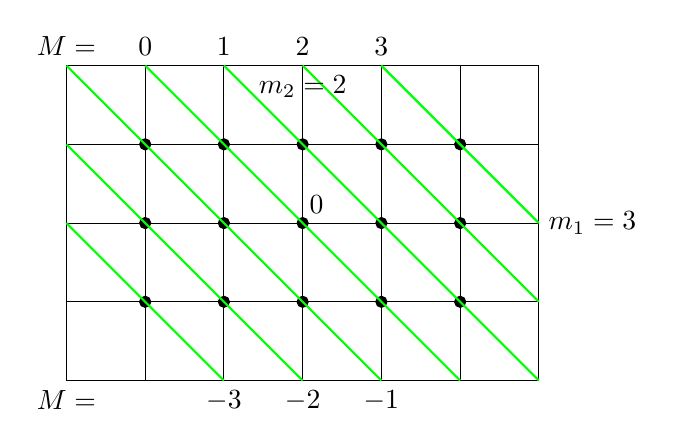
\begin{tikzpicture}[axis/.style={-,thin}]
                \foreach \y in{-2,...,2}
                \draw[axis] (-3,\y) -- +(6,0);
                \foreach \x in{-3,...,3}
                \draw[axis] (\x,-2) -- +(0,4);
                \foreach \x in{-2,...,2}
                {
                    \draw [fill] (\x,1) circle [radius=2pt];
                    \draw [fill] (\x,0) circle [radius=2pt];
                    \draw [fill] (\x,-1) circle [radius=2pt];
                }
                \foreach \y in{0,...,2}
                \draw[thick,green] (-3,\y) -- (-1+\y,-2);
                \foreach \y in{0,...,-2}
                \draw[thick,green] (3,\y) -- (1+\y,2);
                \foreach \y in{3,...,0}
                \draw (\y-2,2) node[above] { \(\y\)};
                \draw (-3,2) node[above] { \(M =\)};
                \foreach \y in{3,2,1}
                \draw (2-\y,-2) node[below] { \( -\y\)};
                \draw (-3,-2) node[below] { \(M =\)};
                \draw[thick,green] (-2,2) -- (2,-2);
                \draw (0,0) node[above] { \(\quad 0\)};
                \draw (3,0) node[right] { \(m_1 = 3\)};
                \draw (0,2) node[below] { \(m_2 = 2\)};
            \end{tikzpicture}
        \end{center}
        There are a total of 15 degrees of freedom. The degree of freedom in each \(M\) subspace is indicated by the number of allowed states (black dots) along the green line. The total lowering operator \(L_ -= L_{1, -} + L_{2, -}\) can be applied to the highest magnetic quantum number state \[
            \ket{L,M} = \ket{3,3} = \ket{2} \ket{1} 
        \] to get the \(L = 3\) states which account for a total of 7 degrees of freedom. For example, \(\ket{3,2} \) can be obtained as \begin{align*}
            \frac{1}{\hbar\sqrt{3}}\pqty{L_{1, -} \otimes I + I \otimes L_{2, - }} \ket{2} \ket{1} &= \frac{1}{\sqrt{6}}\pqty{\sqrt{4} \ket{1} \ket{1}  + \ket{2} \sqrt{2} \ket{0}}\\ 
            \ket{3,2} &= \sqrt{\frac{2}{3}} \ket{1} \ket{1} + \sqrt{\frac{1}{3}} \ket{2} \ket{0}  
        \end{align*}
        Indeed the coefficients are the same as given by Clebsh-Gordan table. The \(\ket{2,2} \) state can then be found as the only state orthogonal to \(\ket{3,2} \) in the 2D \(M = 2\) subspace spanned by \(\ket{1} \ket{1} \) and \(\ket{2} \ket{0} \), \begin{align*}
            \ket{2,2} &= \sqrt{\frac{1}{3}} \ket{1} \ket{1} - \sqrt{\frac{2}{3}} \ket{2} \ket{0} , 
        \end{align*} which can be then lowered to account for \(5\) states with \(L = 2\). Similarly, there are 3 states with \(L = 1\). The table gives \[
            \ket{1, -1} = \sqrt{\frac{1}{10}} \ket{0} \ket{ -1} - \sqrt{\frac{3}{10}} \ket{ -1} \ket{0} + \sqrt{\frac{6}{10}} \ket{ -2} \ket{1}   
        \] All degrees of freedom have been accounted for, so the possible values of \(L\) are \(3,2,1\).
        
        The scalar product of two angular momentum operators can be written as \begin{align*}
            \bf L_1 \cdot \bf L_2 &= L_{1x}  L_{2x} + L_{1y} L_{2y} + L_{1z}L_{2z}\\
            &= \frac{1}{4} (L_{1 +} + L_{1 -}) (L_{2 +} + L_{2 -}) + \frac{1}{4i^2} (L_{1 +} - L_{1 -})(L_{2 +} - L_{2 -}) + L_{1y} L_{2y} + L_{1z}L_{2z}\\
            &= \frac{1}{4} \pqty{L_{1 + }L_{2 -} + L_{1 -}L_{2 +} + L_{1 -}L_{2 +} + L_{1 +}L_{2 -}} + L_{1z} L_{2z}\\
            &= \frac{1}{2} \pqty{L_{1 + }L_{2 -} + L_{1 -}L_{2 + }} + L_{1z} L_{2z}
        \end{align*}
        The square of the total angular momentum operator can be used to verify
        \begin{align*}
            \frac{1}{\hbar^2}\pqty{\bf L_1 +\bf L_2}^2\ket{1, -1} =& \pqty{L_1^2 + L_2^2 + \pqty{L_{1 + }L_{2 -} + L_{1 -}L_{2 + }} + 2L_{1z} L_{2z}}\ket{1, -1}\\
            =& 8\pqty{\sqrt{\frac{1}{10}}  \ket{0} \ket{ -1} - \sqrt{\frac{3}{10}} \ket{ -1} \ket{0} + \sqrt{\frac{6}{10}} \ket{ -2} \ket{1} } \\ 
            &+ \pqty{ -\sqrt{\frac{3}{10}} \sqrt{6}\sqrt{2}\ket{0} \ket{ - 1} + \sqrt{\frac{6}{10}} \sqrt{6 - 2}\sqrt{2}\ket{ - 1} \ket{0}  } \\
            &+\pqty{\sqrt{\frac{1}{10}} \sqrt{6}\sqrt{2}\ket{ - 1} \ket{ 0} - \sqrt{\frac{3}{10}}\sqrt{6 - 2}\sqrt{2} \ket{ - 2} \ket{1}}\\
            &- 4\sqrt{\frac{6}{10}} \ket{ -2} \ket{1}\\
            =& \frac{1}{\sqrt{10}}\left[ \pqty{8 -6 }\ket{0} \ket{ -1} + \pqty{ - 8 \sqrt{3} + \sqrt{48} + \sqrt{12} } \ket{ - 1} \ket{0} + \right. \\
            &\qquad\left. +\pqty{8 \sqrt{6} - \sqrt{24} - 4 \sqrt{6} } \ket{ - 2} \ket{1}  \right]\\
            =& 2 \ket{1, - 1}
            = (L - 1)L \ket{1, - 1}
        \end{align*}
        Similarly \begin{align*}
            &\frac{1}{\hbar} \pqty{L_{1z} + L_{2z}} \ket{1, - 1} \\
            =& (0 - 1)\sqrt{\frac{1}{10}} \ket{0} \ket{ -1} - ( - 1 + 0) \sqrt{\frac{3}{10}} \ket{ -1} \ket{0} + ( - 2 + 1)\sqrt{\frac{6}{10}} \ket{ -2} \ket{1} \\
            =& - 1\ket{1, - 1}
            = - M\ket{1, - 1}
        \end{align*}
        For \(l_1 = 3\) , \(l_2 = 1\), a similar diagram can be plotted \begin{center}
            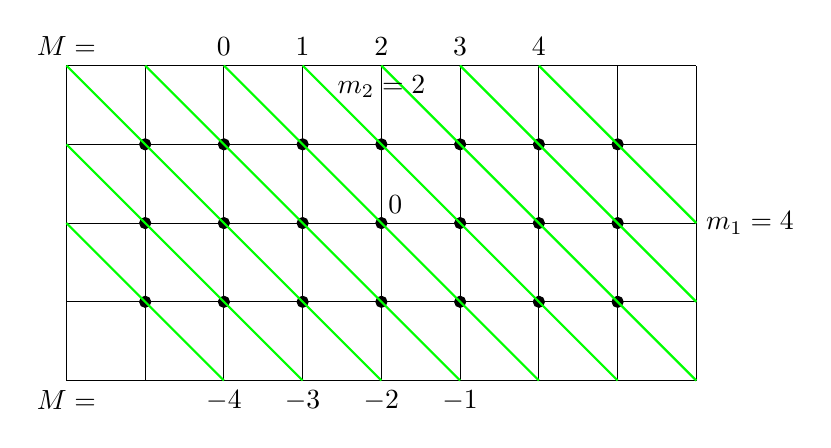
\begin{tikzpicture}[axis/.style={-,thin}]
                \foreach \y in{-2,...,2}
                \draw[axis] (-4,\y) -- +(8,0);
                \foreach \x in{-4,...,4}
                \draw[axis] (\x,-2) -- +(0,4);
                \foreach \x in{-3,...,3}
                {
                    \draw [fill] (\x,1) circle [radius=2pt];
                    \draw [fill] (\x,0) circle [radius=2pt];
                    \draw [fill] (\x,-1) circle [radius=2pt];
                }
                \foreach \y in{-1,...,1}
                \draw[thick,green] (-4,\y+1) -- (-1+\y,-2);
                \foreach \y in{1,...,-1}
                \draw[thick,green] (4,\y-1) -- (1+\y,2);
                \draw[thick,green] (-3,2) -- +(+4,-4);
                \draw[thick,green] (-2,2) -- +(+4,-4);
                \draw[thick,green] (-1,2) -- +(+4,-4);
                \foreach \y in{4,...,0}
                \draw (\y-2,2) node[above] { \(\y\)};
                \draw (-4,2) node[above] { \(M =\)};
                \foreach \y in{4,3,2,1}
                \draw (2-\y,-2) node[below] { \( -\y\)};
                \draw (-4,-2) node[below] { \(M =\)};
                \draw (0,0) node[above] { \(\quad 0\)};
                \draw (4,0) node[right] { \(m_1 = 4\)};
                \draw (0,2) node[below] { \(m_2 = 2\)};
            \end{tikzpicture}
        \end{center}
        The total degrees of freedom is the sum of available states in each ladder 
        \[21 = 9 + 7 + 5\]
        The possible values of total angular momentum are \(L = 4,3,2\).

        Each table in the Clebsh-Gordan coefficients consists of a set of orthonormal vectors which span the subspace of a value of \(M\). By definition, each table makes an orthogonal matrix.
        \subsection{} The Wigner-Eckart theorem states that for a spherical vector (rank-1 tensor) operator \(\hat{\bf V}\) the matrix elements are\[
            \bra{\alpha_1 j_1m_1} \hat{V}_m \ket{\alpha_2j_2m_2} = \bra{\alpha_1j_1} \abs{\hat{\bf V}} \ket{\alpha_2j_2} \bra{1,m;j_2m_2} \ket{j_1m_1}
        \]
        \subsubsection{} For \(j_1 = 1\), \(j_2 = 0\), the Clebsh-Gordan coefficient reduces to simply \[
            \bra{1,m;j_2m_2} \ket{j_1m_1} = \bra{1,m} \ket{j_1,m_1} = \delta_{m,m_1}
        \]
        Therefore, the only possible nonzero spherical components of the operator  \[
            \bra{\alpha_1 1m} \hat{V}_m \ket{\alpha_2 00}
        \]
        all share the same value
        \[
            \bra{\alpha_1j_1} \abs{\hat{\bf V}} \ket{\alpha_2j_2} = A.
        \]
        The spherical components \begin{align*}
            A =\begin{cases}  
                \bra{\alpha_1, 1,0} \hat{V}_z \ket{\alpha_2 00} \\
                \bra{\alpha_1, 1,1} \hat{V}_1 \ket{\alpha_2 00} \\
                \bra{\alpha_1, 1, -1} \hat{V}_{ - 1} \ket{\alpha_2 00} \\
            \end{cases} 
        \end{align*}
        can be transformed into Cartesian components by \begin{align*}
            V_x &= \frac{ -V_1 + V_{ - 1}}{\sqrt{2}} \\
            \bra{\alpha_1, 1, \pm 1} \hat{V}_x \ket{\alpha_2 00} &= \frac{ -\bra{\alpha_1, 1,\pm 1} \hat{V}_1 \ket{\alpha_2 00} + \bra{\alpha_1, 1, \pm 1} \hat{V}_{ -1} \ket{\alpha_2 00}}{\sqrt{2}} \\
            \bra{\alpha_1, 1, \pm 1} \hat{V}_x \ket{\alpha_2 00} &= \frac{A}{\sqrt{2}} \pqty{ -\delta_{1,\pm 1} + \delta_{ - 1,\pm 1}}\\
            \bra{\alpha_1, 1, \pm 1} \hat{V}_x \ket{\alpha_2 00} &= \mp \frac{A}{\sqrt{2}} \\
            V_y &= \frac{V_1 + V_{ - 1}}{ - i \sqrt{2}} \\
            \bra{\alpha_1, 1, \pm 1} \hat{V}_y \ket{\alpha_2 00} &= \frac{ \bra{\alpha_1, 1,\pm 1} \hat{V}_1 \ket{\alpha_2 00} + \bra{\alpha_1, 1, \pm 1} \hat{V}_{ -1} \ket{\alpha_2 00}}{ - i\sqrt{2}} \\
            \bra{\alpha_1, 1, \pm 1} \hat{V}_y \ket{\alpha_2 00} &= i\frac{A}{\sqrt{2}} 
        \end{align*}
        In summary \begin{align*}
            \bra{\alpha_1, 1, 0} \pqty{V_x,V_y,V_z} \ket{\alpha_2 00} &= \pqty{0,0,A}\\
            \bra{\alpha_1, 1, \pm 1} \pqty{V_x,V_y,V_z} \ket{\alpha_2 00} &= \frac{A}{\sqrt{2}} \pqty{\mp 1, i, 0}
        \end{align*}
        \subsubsection{} For a hydrogen-like system, the matrix elements of the position operator related to transition between \(j = 0\) and \(j = 1\) are \begin{align*}
            &\bra{\alpha 1m} \hat{\bf r} \ket{\alpha 00} \\
            =& \int_0^{\infty} R^*_{\alpha 1} (r) R_{\alpha 0}(r) r^3 \dd{r} \int_0^{2\pi} \int_0^\pi Y^*_{1m}(\theta,\phi)  Y_{00}(\theta,\phi)  \begin{pmatrix} \sin\theta\cos\phi\\ \sin\theta \sin\phi\\ \cos\theta \end{pmatrix} \sin\theta \dd{\theta}   \dd{\phi}\\
            =&B_{\alpha_1,\alpha_0} \frac{1}{\sqrt{4\pi}}\int_0^{2\pi} \int_0^\pi Y^*_{1m}(\theta,\phi)   \begin{pmatrix} \sin\theta\cos\phi\\ \sin\theta \sin\phi\\ \cos\theta \end{pmatrix} \sin\theta \dd{\theta}   \dd{\phi}   
        \end{align*} 
        where we denoted \(\int_0^{\infty} R^*_{\alpha 1} (r) R_{\alpha 0}(r) r^3 \dd{r} =B_{\alpha_1,\alpha_0}\) for simplicity, substituting in \(m =\pm 1,0\), we get
        \begin{align*}
            \bra{\alpha,1,\pm 1} \hat{\bf r} \ket{\alpha, 0,0} &=  \frac{B_{\alpha_1,\alpha_0}}{4\pi}  \int_0^{2\pi} \int_0^\pi \mp \sqrt{\frac{3}{2}} \sin\theta e^{ \mp i\phi}   \begin{pmatrix} \sin\theta\cos\phi\\ \sin\theta \sin\phi\\ \cos\theta \end{pmatrix} \sin\theta \dd{\theta}   \dd{\phi}  \\
            &=  \mp \sqrt{\frac{3}{2}} \frac{B_{\alpha_1,\alpha_0}}{4\pi}  \int_0^{2\pi} \int_0^\pi   \begin{pmatrix} e^{ \mp i\phi}\sin^3\theta\cos\phi\\ e^{ \mp i\phi}\sin^3\theta \sin\phi\\ e^{ \mp i\phi}\cos\theta \sin^2\theta \end{pmatrix} \dd{\theta}   \dd{\phi}  \\
            &=  \mp \sqrt{\frac{3}{2}} \frac{B_{\alpha_1,\alpha_0}}{2}  \int_0^\pi   \begin{pmatrix} \frac{1}{2}\sin^3\theta\\ \pm \frac{1}{2i}\sin^3\theta \\ 0\end{pmatrix} \dd{\theta}   \\
            &=  \frac{1}{\sqrt{2}}\frac{B_{\alpha_1,\alpha_0}}{\sqrt{3}}  \begin{pmatrix} \mp 1\\ i\\0 \end{pmatrix}\\ 
            \bra{\alpha,1,0} \hat{\bf r} \ket{\alpha, 0,0} &=  \frac{B_{\alpha_1,\alpha_0}}{4\pi}  \int_0^{2\pi} \int_0^\pi \sqrt{3} \cos\theta  \begin{pmatrix} \sin\theta\cos\phi\\ \sin\theta \sin\phi\\ \cos\theta \end{pmatrix} \sin\theta \dd{\theta}   \dd{\phi}  \\
            &=  \sqrt{3} \frac{B_{\alpha_1,\alpha_0}}{2}\int_0^\pi   \begin{pmatrix} 0 \\ 0\\ \sin\theta \cos^2\theta \end{pmatrix}  \dd{\theta}    \\
            &=  \frac{B_{\alpha_1,\alpha_0}}{\sqrt{3}}\begin{pmatrix} 0\\0\\ 1 \end{pmatrix} 
        \end{align*}
        As expected from Wigner-Eckart theorem, with \(A = \frac{B_{\alpha_1,\alpha_0}}{\sqrt{3}}\).
        \subsubsection{} For \(j_1 = j_2 = 0\), the inner product \(\bra{1,m} \ket{0,0} = 0\) always. There are no nonzero elements of \(\hat{\bf V}\) in this subspace.
        \subsection{} 
        \subsubsection{} The perturbation applied on a hydrogen atom by a uniform external field is \[
            \hat{H}' = e \mathcal{E} \hat{z}
        \]
        Wigner-Eckart theorem tells us, on the level \(n = 3\) \[
            \bra{3lm} e\mathcal{E} z \ket{3l'm'} = \bra{3l} \abs{\hat{\bf r}} \ket{3l'} e \mathcal{E} \bra{10;l'm'} \ket{lm}
        \]
        Nonzero Clebsh-Gordan coefficients require \(m' + 0 = m\). Therefore, the operator \(\hat{H}'\) is block-diagonal when grouped according to different values of \(m\). Using the Hermitianity of \(\hat{H}'\), the only nonzero Clebsh-Gordan coefficients that need to be found are \begin{align*}
            \bra{10;10} \ket{00} = - \sqrt{\frac{1}{3}} \qquad\bra{10;10} \ket{20} = \sqrt{\frac{2}{3}}\qquad\bra{10;1,\pm 1} \ket{2,\pm 1} = \sqrt{\frac{1}{2}}
        \end{align*}
        which, along with the reduced matrix elements \[\bra{30}\abs{\hat{\bf r}} \ket{31} = 9 \sqrt{2} a_0\qquad\text{and}\qquad\bra{32}\abs{\hat{\bf r}} \ket{31} =- \frac{9}{\sqrt{2}}a_0\] gives \begin{align*}
            H'_0 &= e\mathcal{E}a_0 \begin{pmatrix} &- \frac{9}{2} \sqrt{\frac{8}{3}}&\\ - \frac{9}{2} \sqrt{\frac{8}{3}}&&- \frac{9}{2 \sqrt{2}} \sqrt{\frac{8}{3}}\\& - \frac{9}{2 \sqrt{2}} \sqrt{\frac{8}{3}} \end{pmatrix}\\
            H'_{\pm 1} &= e\mathcal{E}a_0 \begin{pmatrix} &- \frac{9}{2}\\ - \frac{9}{2}&\end{pmatrix}& H'_{\pm 2} = 0
        \end{align*}
        \subsubsection{} Diagonalising these submatrices, we first find \(\hat{H}'_{\pm 1}\) both split the unpertubed energy by \(\pm \frac{9}{2} e \mathcal{E}a_0 =\pm E_d\). 

        The submatric \(H'_0\) has eigenvalues \(\lambda E_d\) which satisfy \begin{align*}
            0 &= - \lambda\bqty{\lambda^2 - \pqty{\frac{2}{\sqrt{3}}}^2} + \pqty{\sqrt{\frac{8}{3}}}^2 \lambda\\
            \lambda &= \begin{cases}
                0\\
                \pm \sqrt{\frac{4}{3} + \frac{8}{3}} =\pm 2
            \end{cases}
        \end{align*}
        So the \(m = 0\) subspace is split into three energies.

        In summary, the 9D degenerate \(n = 3\) subspace is split by a perturbing field into 5 energy levels \[
            \Delta  E = \begin{cases}
                + 2 E_d \qquad m_l = 0&\text{nondegenerate}\\
                + 1 E_d \qquad m_l =\pm 1&\text{twofold degenerate}\\
                + 0E_d\qquad m_l = \pm 2, 0 &\text{threefold degenerate}\\
                - 1 E_d \qquad m_l =\pm 1&\text{twofold degenerate}\\
                - 2 E_d \qquad m_l = 0&\text{nondegenerate}\\
            \end{cases}
        \]
        where \(E_d = \frac{9}{2} e \mathcal{E}a_0\) 
        \subsubsection{} The highest perturbed energy level in \(n = 3\), with \(\Delta E = + 2 E_d\), satisfies the energy eigenvalue equation \begin{align*}
            + 2 \begin{pmatrix} a_1\\ a_2\\a_3 \end{pmatrix} &= \begin{pmatrix} &-\sqrt{\frac{8}{3}}&\\ -\sqrt{\frac{8}{3}}&& -\sqrt{\frac{4}{3}}\\& - \sqrt{\frac{4}{3}} \end{pmatrix} \begin{pmatrix} a_1\\a_2\\a_3 \end{pmatrix} \\
            \ket{\psi} &= \begin{pmatrix} \ket{300} &\ket{310} &\ket{320}  \end{pmatrix}  \begin{pmatrix} 1\\- \sqrt{\frac{3}{2}}\\ \sqrt{\frac{1}{2}} \end{pmatrix} a_1\\
            \ket{\psi} &= \sqrt{\frac{1}{3}} \ket{300} - \sqrt{\frac{1}{2}} \ket{310} + \sqrt{\frac{1}{6}} \ket{320} .
        \end{align*}
        \subsection{} Identical to Qu. 6 on example sheet 1.
        \subsection{} The observed conductance oscillates periodically because the interference of electron wavefunctions are shifted by the varied magentic flux through the loop. Conductance maxima are measured when the electrons arriving from opposite parts of the loop are in phase, and minima when they are out of phase. Aharanov-Bohm effect relates phase difference of two paths to the magnetic flux enclosed. The total number of oscillations over a change of field strength by \(10^3\) Gauss is \(32\), so the diameter of the ring can be estimated as
        \begin{align*}
            \frac{e\Phi}{\hbar} &= \delta \\
            \frac{eB d^2}{8\hbar} &= 32\\ 
            d &= 1.30 \; \mathrm{\mu m}.
        \end{align*}

\end{document}